This manuscript
(\href{https://SORTEE-Github-Hackathon.github.io/manuscript/v/659dbf07d94474726c8403d04555afbb3a45da57/}{permalink})
was automatically generated
from \href{https://github.com/SORTEE-Github-Hackathon/manuscript/tree/659dbf07d94474726c8403d04555afbb3a45da57}{SORTEE-Github-Hackathon/manuscript@659dbf0}
on February 6, 2023.

\hypertarget{authors}{%
\subsection{Authors}\label{authors}}

\begin{itemize}
\item
  \textbf{Robert Crystal-Ornelas}
  
\includegraphics[width=0.16667in,height=0.16667in]{images/orcid.svg}
  \href{https://orcid.org/0000-0002-6339-1139}{0000-0002-6339-1139}
  · 
\includegraphics[width=0.16667in,height=0.16667in]{images/github.svg}
  \href{https://github.com/robcrystalornelas}{robcrystalornelas}
  · 
\includegraphics[width=0.16667in,height=0.16667in]{images/twitter.svg}
  \href{https://twitter.com/rob_c_ornelas}{rob\_c\_ornelas}
  Earth and Environmental Sciences Area, Lawrence Berkeley National Laboratory, Berkeley, CA 94720, USA
\item
  \textbf{Brandon P.M. Edwards}
  
\includegraphics[width=0.16667in,height=0.16667in]{images/orcid.svg}
  \href{https://orcid.org/0000-0003-0865-3076}{0000-0003-0865-3076}
  · 
\includegraphics[width=0.16667in,height=0.16667in]{images/github.svg}
  \href{https://github.com/BrandonEdwards}{BrandonEdwards}
  Department of Biology, Carleton University, Ottawa, ON K1S 5B6, Canada
\item
  \textbf{Katherine Hébert}
  
\includegraphics[width=0.16667in,height=0.16667in]{images/orcid.svg}
  \href{https://orcid.org/0000-0001-7866-6775}{0000-0001-7866-6775}
  · 
\includegraphics[width=0.16667in,height=0.16667in]{images/github.svg}
  \href{https://github.com/katherinehebert}{katherinehebert}
  · 
\includegraphics[width=0.16667in,height=0.16667in]{images/twitter.svg}
  \href{https://twitter.com/hebert_kat}{hebert\_kat}
  Département de biologie, Université de Sherbrooke, Québec, Canada
\item
  \textbf{Emma J. Hudgins}
  
\includegraphics[width=0.16667in,height=0.16667in]{images/orcid.svg}
  \href{https://orcid.org/0000-0002-8402-5111}{0000-0002-8402-5111}
  · 
\includegraphics[width=0.16667in,height=0.16667in]{images/github.svg}
  \href{https://github.com/emmajhudgins}{emmajhudgins}
  Department of Biology, Carleton University, Ottawa, ON K1S 5B6, Canada
\item
  \textbf{Luna L. Sánchez Reyes}
  
\includegraphics[width=0.16667in,height=0.16667in]{images/orcid.svg}
  \href{https://orcid.org/0000-0001-7668-2528}{0000-0001-7668-2528}
  · 
\includegraphics[width=0.16667in,height=0.16667in]{images/github.svg}
  \href{https://github.com/LunaSare}{LunaSare}
  · 
\includegraphics[width=0.16667in,height=0.16667in]{images/twitter.svg}
  \href{https://twitter.com/LunaSare}{LunaSare}
  School of Natural Sciences, University of California, Merced, USA
\item
  \textbf{Eric R. Scott}
  
\includegraphics[width=0.16667in,height=0.16667in]{images/orcid.svg}
  \href{https://orcid.org/0000-0002-7430-7879}{0000-0002-7430-7879}
  · 
\includegraphics[width=0.16667in,height=0.16667in]{images/github.svg}
  \href{https://github.com/Aariq}{Aariq}
  Department of Wildlife Ecology and Conservation, University of Florida, Gainesville, FL, USA
\item
  \textbf{Matthew J. Grainger}
  
\includegraphics[width=0.16667in,height=0.16667in]{images/orcid.svg}
  \href{https://orcid.org/0000-0001-8426-6495}{0000-0001-8426-6495}
  · 
\includegraphics[width=0.16667in,height=0.16667in]{images/github.svg}
  \href{https://github.com/DrMattG}{DrMattG}
  · 
\includegraphics[width=0.16667in,height=0.16667in]{images/twitter.svg}
  \href{https://twitter.com/Ed_pheasant}{Ed\_pheasant}
  Terrestrial Biodiversity, Norwegian Institute for Nature Research - NINA, Postbox 5685 Torgarden, 7485 Trondheim, Norway
\item
  \textbf{Vivienne Foroughirad}
  
\includegraphics[width=0.16667in,height=0.16667in]{images/orcid.svg}
  \href{https://orcid.org/0000-0002-8656-7440}{0000-0002-8656-7440}
  · 
\includegraphics[width=0.16667in,height=0.16667in]{images/github.svg}
  \href{https://github.com/vjf2}{vjf2}
  · 
\includegraphics[width=0.16667in,height=0.16667in]{images/twitter.svg}
  \href{https://twitter.com/vforoughirad}{vforoughirad}
  Department of Biology, Georgetown University, Washington, DC, USA
\item
  \textbf{Allison D. Binley}
  
\includegraphics[width=0.16667in,height=0.16667in]{images/orcid.svg}
  \href{https://orcid.org/0000-0001-8790-9935}{0000-0001-8790-9935}
  · 
\includegraphics[width=0.16667in,height=0.16667in]{images/github.svg}
  \href{https://github.com/adbinley}{adbinley}
  · 
\includegraphics[width=0.16667in,height=0.16667in]{images/twitter.svg}
  \href{https://twitter.com/AllisonBinley}{AllisonBinley}
  Department of Biology, Carleton University, Ottawa, ON K1S 5B6, Canada
\item
  \textbf{Cole B. Brookson}
  
\includegraphics[width=0.16667in,height=0.16667in]{images/orcid.svg}
  \href{https://orcid.org/0000-0003-1237-4096}{0000-0003-1237-4096}
  · 
\includegraphics[width=0.16667in,height=0.16667in]{images/github.svg}
  \href{https://github.com/colebrookson}{colebrookson}
  Department of Biological Sciences, University of Alberta, Edmonton, AB, Canada
\item
  \textbf{Kaitlyn M. Gaynor}
  
\includegraphics[width=0.16667in,height=0.16667in]{images/orcid.svg}
  \href{https://orcid.org/0000-0002-5747-0543}{0000-0002-5747-0543}
  · 
\includegraphics[width=0.16667in,height=0.16667in]{images/github.svg}
  \href{https://github.com/kaitlyngaynor}{kaitlyngaynor}
  · 
\includegraphics[width=0.16667in,height=0.16667in]{images/twitter.svg}
  \href{https://twitter.com/kaitlyngaynor}{kaitlyngaynor}
  Departments of Zoology and Botany, University of British Columbia, Vancouver, BC, Canada; National Center for Ecological Analysis and Synthesis, Santa Barbara, CA 93101, USA
\item
  \textbf{Saeed Shafiei Sabet}
  
\includegraphics[width=0.16667in,height=0.16667in]{images/orcid.svg}
  \href{https://orcid.org/0000-0001-5919-2527}{0000-0001-5919-2527}
  · 
\includegraphics[width=0.16667in,height=0.16667in]{images/github.svg}
  \href{https://github.com/shafieisabets}{shafieisabets}
  · 
\includegraphics[width=0.16667in,height=0.16667in]{images/twitter.svg}
  \href{https://twitter.com/SaeedSHSABET}{SaeedSHSABET}
  Fisheries Department, Faculty of Natural Resources, University of Guilan, Sowmeh Sara, Iran
\item
  \textbf{Ali Güncan}
  
\includegraphics[width=0.16667in,height=0.16667in]{images/orcid.svg}
  \href{https://orcid.org/0000-0003-1765-648X}{0000-0003-1765-648X}
  · 
\includegraphics[width=0.16667in,height=0.16667in]{images/github.svg}
  \href{https://github.com/Aguncan}{Aguncan}
  · 
\includegraphics[width=0.16667in,height=0.16667in]{images/twitter.svg}
  \href{https://twitter.com/aliguncan}{aliguncan}
  Department of Plant Protection, Faculty of Agriculture, Ordu University, 52200, Ordu, Turkey
\item
  \textbf{Friederike Hillemann}
  
\includegraphics[width=0.16667in,height=0.16667in]{images/orcid.svg}
  \href{https://orcid.org/0000-0002-8992-0676}{0000-0002-8992-0676}
  · 
\includegraphics[width=0.16667in,height=0.16667in]{images/github.svg}
  \href{https://github.com/fhillemann}{fhillemann}
  Department of Human Behavior, Ecology and Culture, Max Planck Institute for Evolutionary Anthropology, Leipzig, Germany
\item
  \textbf{Helen Weierbach}
  
\includegraphics[width=0.16667in,height=0.16667in]{images/orcid.svg}
  \href{https://orcid.org/0000-0001-6348-9120}{0000-0001-6348-9120}
  · 
\includegraphics[width=0.16667in,height=0.16667in]{images/github.svg}
  \href{https://github.com/helenweierbach}{helenweierbach}
  · 
\includegraphics[width=0.16667in,height=0.16667in]{images/twitter.svg}
  \href{https://twitter.com/HWeierbach}{HWeierbach}
  Earth and Environmental Sciences Area, Lawrence Berkeley National Laboratory, Berkeley, CA 94720, USA
\item
  \textbf{Dylan G. E. Gomes}
  
\includegraphics[width=0.16667in,height=0.16667in]{images/orcid.svg}
  \href{https://orcid.org/0000-0002-2642-3728}{0000-0002-2642-3728}
  · 
\includegraphics[width=0.16667in,height=0.16667in]{images/github.svg}
  \href{https://github.com/dylangomes}{dylangomes}
  (Current) National Academy of Sciences NRC Research Associateship Program, Northwest Fisheries Science Center, National Marine Fisheries Service, National Oceanic and Atmospheric Administration, Seattle, WA, USA 98112; (Former) Cooperative Institute for Marine Resources Studies, Hatfield Marine Science Center, Oregon State University, Newport, OR, USA 97365
\item
  \textbf{Pedro Henrique Pereira Braga}
  
\includegraphics[width=0.16667in,height=0.16667in]{images/orcid.svg}
  \href{https://orcid.org/0000-0002-1308-1562}{0000-0002-1308-1562}
  · 
\includegraphics[width=0.16667in,height=0.16667in]{images/github.svg}
  \href{https://github.com/pedrohbraga}{pedrohbraga}
  · 
\includegraphics[width=0.16667in,height=0.16667in]{images/twitter.svg}
  \href{https://twitter.com/pedrohp_braga}{pedrohp\_braga}
  Department of Biology, Concordia University, 7141 Sherbrooke Street West, Montreal, QC H4B 1R6, Canada
\end{itemize}

\hypertarget{abstract}{%
\subsection{Abstract}\label{abstract}}

Researchers in ecology and evolutionary biology are increasingly dependent on computational code to conduct research, and the use of efficient methods to share, reproduce, and collaborate on code as well as any research-related documentation has become fundamental.
GitHub is an online, cloud-based service that can help researchers track, organize, discuss, share, and collaborate on software and other materials related to research production, including data, code for analyses, and protocols.

Despite these benefits, the use of GitHub in ecology and evolution is not widespread.
To help researchers in ecology and evolution adopt useful features from GitHub in their own workflows, we review twelve practical ways to use the platform.
We outline features ranging from low to high technical difficulty: storing code, managing projects, coding collaboratively, conducting peer review, and writing a manuscript.
Given that members of a research team may have different technical skills and responsibilities, we describe how the optimal use of GitHub features may vary among members of a research collaboration.
As more ecologists and evolutionary biologists establish their workflows using GitHub, the field can continue to push the boundaries of collaborative, transparent, and open research.

\hypertarget{introduction}{%
\subsection{Introduction}\label{introduction}}

Most scientists, including ecologists and evolutionary biologists, depend on computational tools for their research (\protect\hyperlink{ref-fJWFe93e}{Hannay et al., 2009}).
Researchers write and use software packages or write code (hereafter, code) to perform scientific tasks ranging from data management, data analysis, and study replication, to the application and the development of tools for hypothesis testing.
Maintaining code for scientific collaboration requires an efficient and well-documented work-flow (\protect\hyperlink{ref-1Kqna6l2}{J. M. Perkel, 2020}).
To facilitate this process, scientists have been adopting tools from information and systems technology, such as cloud-based services for documentation and version control {[}\emph{e.g.}, the Google Suite, the Microsoft Suite, DropBox, and GitHub (\protect\hyperlink{ref-10ghgV3S8}{J. Perkel, 2016}){]}.
Of all the tools mentioned above, GitHub is uniquely positioned (\protect\hyperlink{tbl:compare}{Table 1}) to benefit scientists because the platform is designed to enable collaboration on computer code--a fundamental component of modern research.
However, most researchers lack exposure to adequate code practices and thus dedicate valuable time and effort to self-teaching research-facilitating tools.
GitHub is one of the most used web-based platforms for computational version control and collaboration, and in this paper we provide researchers in ecology and evolutionary biology (EEB) with practical workflows to use GitHub to facilitate and improve their code and its management.

GitHub (\url{https://github.com}) provides a simple but powerful web interface that allows users to participate in projects by contributing, modifying and discussing existing code, reporting bugs, discovering code and data, and publishing new code.
Through version control, users have a detailed, chronological record of the files and directories stored in their repositories (\protect\hyperlink{ref-RVetqmsg}{Bryan, 2018}) (see \protect\hyperlink{definitions}{Box 1}).
Additionally, unlike sharing documents and code via DropBox or Google Drive links, GitHub defaults to public sharing of code and documents and has features like Issues and Discussions (see \protect\hyperlink{definitions}{Box 1}) that can immediately and directly contribute to more open science and knowledge sharing.
This workflow provides a strong and clear advantage over sending files back-and-forth (\emph{e.g.}, via email), a process that can become challenging and time-consuming in long-term and collaborative projects (\protect\hyperlink{ref-4ny1onB0}{Ram, 2013}).
Through its combination of version control and collaborative features, GitHub facilitates open-source code alongside collaborative development (\protect\hyperlink{ref-kEX5dgzK}{Perez-Riverol et al., 2016}).

Git is the version control system that enables all the collaborative tools available on GitHub.
Git was originally developed as a fast, lightweight and open-source system that would allow software engineers to efficiently develop and collaborate in projects (\protect\hyperlink{ref-1CM2EcdVk}{\emph{Git - A Short History of Git}, n.d.}).
Since its launch in 2005, Git has become the leading version control system in software development and in other disciplines that similarly require collaboration and community contributions, such as scientific research (\protect\hyperlink{ref-7q3wZN6d}{Spinellis, 2012}).
Although the understanding of basic concepts of Git (such as commit, push, pull, checkout; see \protect\hyperlink{definitions}{Box 1}) is necessary, the GitHub web-based platform and its integrated development environments (such as GitHub Desktop) allow users to perform most repository and data management operations without opening Git command-line sessions, making these functionalities available to users who are less familiar with software development.

Version control involves tracking the state of the files in a folder, called a ``repository'' (see \protect\hyperlink{definitions}{Box 1}), through the evolution of a project.
A basic workflow using git and GitHub is to 1) make changes to files in a repository on your computer, 2) record related changes in files as a ``commit'' (see \protect\hyperlink{definitions}{Box 1}) along with a message describing the changes, 3) synchronize commits with GitHub (see ``push'' in \protect\hyperlink{definitions}{Box 1}) so that the repository on the web is up to date.
Collaborators can then view your changes online and synchronize them to their own computers (see ``pull'' in \protect\hyperlink{definitions}{Box 1}).
Commits act like snapshots and one can view or even revert the state of the project to any previous commit.
If the modified files are plain text (\emph{e.g.} computer code or .txt files), only the differences from the previous commit are recorded, allowing you to frequently commit changes without causing the size of the project to grow excessively.
This provides a safe and less cluttered alternative to frequently making full copies of documents at different points in their evolution (\emph{e.g.} analysis.R, analasys\_v2.R, analysis\_FINAL.R).
More technical details about the use of Git and GitHub are beyond the scope of this paper (but see Perez-Riverol et al. (\protect\hyperlink{ref-kEX5dgzK}{2016}), Blischak et al. (\protect\hyperlink{ref-PlcxShQU}{2016}), and Kalliamvakou et al. (\protect\hyperlink{ref-ndfO9H}{2015})).

The expansive GitHub user-community and numerous GitHub resources have boosted its popularity {[}Perez-Riverol et al. (\protect\hyperlink{ref-kEX5dgzK}{2016}); Bryan (\protect\hyperlink{ref-RVetqmsg}{2018}); \url{https://happygitwithr.com}; \url{https://ourcodingclub.github.io}{]}.
Nevertheless, although multiple articles have encouraged researchers in EEB to adopt GitHub as part of their research process (\protect\hyperlink{ref-3DKwn1sY}{Lowndes et al., 2017}; \protect\hyperlink{ref-10ghgV3S8}{J. Perkel, 2016}), its use is still not widespread.
First-time users without formal training in information technology may face steep learning curves because GitHub and its features have been centered on software development (\protect\hyperlink{ref-139b0pSGc}{Leibzon, 2016}).
Moreover, domain-specific resources providing tractable examples and practical guidance for researchers in EEB on GitHub are scarce {[}but see Kim et al. (\protect\hyperlink{ref-lJAgyhYq}{2022}); \url{https://ourcodingclub.github.io}; \url{https://www.openscapes.org}{]}.
Widespread adoption of GitHub for collaborating on research tasks can ultimately enable EEB researchers to spend less time on creating novel processes for collaboration and more time on their research (\protect\hyperlink{ref-ydrk01SR}{Briney et al., 2020}).
More importantly, expanding the availability of data and code management standards---of which GitHub is one increasingly important component---makes research more reproducible and collaborative (\protect\hyperlink{ref-13QX8XU3J}{Alston \& Rick, 2021}; \protect\hyperlink{ref-pq2Tv1BC}{Gomes et al., 2022b}).

This paper is the result of an academic hackathon held during the 2021 conference for the Society for Open, Reliable, and Transparent Ecology and Evolutionary Biology (SORTEE, \url{https://www.sortee.org}).
We convened around thirty researchers in EEB with varying levels of familiarity with the usage of GitHub in research projects to showcase and discuss how existing features can contribute to documentation and collaboration in EEB research.
During the hackathon, we identified the need for formal discussions on how EEB researchers can benefit from GitHub and its features.
Here, we outline twelve practical ways that EEB researchers can use GitHub features for more collaborative, transparent, and reproducible science.
We also provide critical perspectives on features that could be improved and catered towards research development.

\hypertarget{definitions}{%
\subsubsection{Box 1}\label{definitions}}

\begin{tablenos:no-prefix-table-caption}

\begin{longtable}[]{@{}
  >{\raggedright\arraybackslash}p{(\columnwidth - 0\tabcolsep) * \real{1.0000}}@{}}
\toprule
\begin{minipage}[b]{\linewidth}\raggedright
Glossary
\end{minipage} \\
\midrule
\endhead
\textbf{repository}: A repository (commonly shortened to ``repo'') is a collection of files (\emph{e.g.}, a directory) tracked by Git. Repositories are managed by an owner and can be made either ``public'', to be visible to all GitHub users, or ``private'', to selected owner-specified users. Repositories can be either ``local'' and saved on an individual's computer or ``remote'' and stored on the cloud via GitHub's web platform. \\
\textbf{fork}: A fork is a copy of a \textbf{repository} hosted on GitHub. If a repository is public, then anyone can make a fork. Even if they do not have access to \textbf{push} to the original repository, they can make a fork and edit it independently. Forks are linked to the original GitHub repository and ``upstream'' changes (\emph{i.e.}, those in the original repository) can be \textbf{merged} to keep the fork up-to-date with the original project. Changes made in the fork can be integrated into the original project via \textbf{pull requests}. \\
\textbf{clone}: Cloning a \textbf{repository} is a way of making a local copy (\emph{i.e.}, on your computer) of a GitHub \textbf{repository}. If you have access to \textbf{push} to a \textbf{repository}, this can be a first step to contributing to a project. \\
\textbf{branch}: Git workflow timelines or repositories are analogous to trees, with a main working project and diverging branches that are pointers to changes during the development process. A git branch is an alternative line of development for a project (repository). Branches allow users to add new features or modifications to the project without affecting the main part of the project. Development branches can be created at any point in time and work on each branch can continue independently. Branching is useful for testing out new ideas (both code and text) which may or may not eventually get integrated into the main branch of the project. Branches can also be used to isolate contributions of multiple contributors. Each person working on their own branch eliminates problems that may arise if conflicting edits are \textbf{pushed} to the same remote branch. Changes in a development branch can be \textbf{merged} into the main branch via \textbf{pull requests}. Branches can only be made by those who are given access to the project \textbf{repository}. \\
\textbf{commit}: Commits are snapshots of the development of a project. In Git, versions of files and directories are uniquely identified as ``commits'', allowing one to identify and track modifications line-by-line. Commits can include changes in multiple files and must include a brief commit message describing the changes made. A typical workflow is to make some related changes in files, add a commit message (\emph{e.g.}, ``Generate and include results figure''), and after several commits \textbf{push} those commits to the remote (\emph{i.e.}, cloud-based) GitHub \textbf{repository}. \\
\textbf{push and pull}: When \textbf{commits} are made in a project locally, they must be synced with the remote GitHub repository by \textbf{pushing} them. Changes on a GitHub repository can then be \textbf{pulled} to keep your local version of the project up-to-date with the remote. \\
\textbf{pull request}: A pull request is a request for changes made on an individual's \textbf{branch} in the repository or in a user's \textbf{fork} to be merged to the repository. Pull requests contain a description of the changes alongside all code required for testing and review by other users prior to being merged into the repository. \\
\textbf{merge}: Combining \textbf{commits} from two different branches together into one \textbf{branch}. \\
\textbf{release}: At any point a release can be made on GitHub to mark a significant milestone in the progression of a \textbf{repository}. While this GitHub feature is designed with releases of new versions of code in mind (\emph{e.g.}, v1.0.0), it can also be used to create a snapshot of a repository at significant stages like pre-print, submission, revision, and acceptance of an associated manuscript. \\
\textbf{community}: A forum where GitHub users can ask for advice, offer solutions to questions, and share ideas (\url{https://github.community/}). \\
\bottomrule
\end{longtable}

\end{tablenos:no-prefix-table-caption}

\hypertarget{twelve-practical-ways-github-can-accelerate-research-in-ecology-and-evolution}{%
\subsection{Twelve practical ways GitHub can accelerate research in ecology and evolution}\label{twelve-practical-ways-github-can-accelerate-research-in-ecology-and-evolution}}

\hypertarget{storing-and-sharing-research-compendia}{%
\subsubsection{Storing and sharing research compendia}\label{storing-and-sharing-research-compendia}}

An EEB research compendium includes all computational materials related to research production, including data, code for analyses and protocols.
Safely storing these files is essential to protect against accidental modifications or deletions.
Many researchers begin using GitHub to backup their research compendium (\protect\hyperlink{ref-MwwMapRG}{Marwick et al., 2018}) into a centralized, readily-available remote server (see \protect\hyperlink{definitions}{Box 1}).
A centralized research compendium stored in a version-controlled repository has the advantages of facilitating collaboration, integrating data and code archiving, allowing file versions to be accessed and restored, and further contributing to open science practices (Borghi \& Van Gulick (\protect\hyperlink{ref-gLby7jt1}{2022})).
Every change made to files in a version-controlled repository accompany a description of modifications and are authored (\protect\hyperlink{definitions}{Box 1}).
Later, the entire history of commits and their commit messages are viewable and can be audited similar to a physical laboratory notebook (\protect\hyperlink{ref-4ny1onB0}{Ram, 2013}).
On GitHub, code can be made public, and the process of forking and submitting pull requests (see \protect\hyperlink{definitions}{Box 1}) ensures code owners have full control over code and documents in a repository.
The ability to make a GitHub repository private is particularly advantageous for storing materials without necessarily sacrificing privacy, which may be preferred or even essential for certain compendia.
Researchers can then grant specific collaborators read and/or write access to private repositories to pursue pre-publication analyses or writing in privacy, or even to collaborate on research that will permanently remain private.

GitHub limits committed file sizes to 100 Mb (megabytes) (\protect\hyperlink{ref-1Co6ZZjF1}{\emph{About Large Files on GitHub}, n.d.}), which can may require external file storage alternatives (such as local or cloud-hosting) for some parts of research compendia.
However, with some additional setup, users can still track versions of these external files in their repositories using Git Large File Storage (\url{https://git-lfs.github.com}).

\hypertarget{project-continuity}{%
\subsubsection{Project continuity}\label{project-continuity}}

Projects in ecology and evolution often involve research professionals holding limited-term positions, such as graduate students, research assistants, and post-doctoral fellows (\protect\hyperlink{ref-D4C4k4ak}{Fehr et al., 2021}).
Without clear plans on project continuity, the research code and data management upkeep tend to fall off as researchers move on to new projects or other institutions.
Additionally, code and data can be difficult to access when kept only on personal devices (\protect\hyperlink{ref-19kmNxiHc}{Vines et al., 2014}).

GitHub can facilitate project continuity among research code by making code handover easier (\protect\hyperlink{ref-D4C4k4ak}{Fehr et al., 2021}; \protect\hyperlink{ref-4ny1onB0}{Ram, 2013}).
Through version control, the history of code and data from projects in ecology and evolution can be tracked accessible to future laboratory members and collaborators (\protect\hyperlink{ref-3DKwn1sY}{Lowndes et al., 2017}).
Repositories and organizations can have designated data and code owners {[}or more appropriate, stewards; see Hampton et al. (\protect\hyperlink{ref-iIEKCTLU}{2015}), \emph{About Code Owners} (\protect\hyperlink{ref-s91uGRZ2}{n.d.}){]}, who can also change through time allowing for the transition of code between research cohorts (see also \protect\hyperlink{organizations}{``Organizing and managing teams''}).
Other project collaborators can contribute to repository design and development, and their active involvement can both aid authors ability to act as guarantors of the project, and the clarity and reproducibility of the project for future users.
In (Figure \ref{fig:github-diagram}), we highlight several elements of good repository structure, and the various ways that contributors may interact with them.

GitHub also allows users to describe and store information about software and code dependencies, ensuring that code can run using the same version of software as when it was initially developed.
This can be achieved through the access of GitHub repositories containing the necessary releases of such software, or through the use of automated Github Actions with specific software versions.

GitHub can facilitate lab continuity by being used as a platform for storing, selectively sharing, and easily updating lab policies and experimental protocols.
Researchers have been increasingly using GitHub to maintain versions and share digital laboratory handbooks across many fields (\protect\hyperlink{ref-10ghgV3S8}{J. Perkel, 2016}), including applied ecology (\emph{e.g.}, \url{https://scheuerell-lab.github.io/lab-book}), biogeography and global change biology (\emph{e.g.}, \url{https://github.com/HuckleyLab/how_we_work}), and microbial ecology (\emph{e.g.}, \url{https://github.com/CarBBAS/uqam-guide}).

\hypertarget{project-management}{%
\subsubsection{Project management}\label{project-management}}

Modern research in ecology and evolution is highly collaborative, bringing together multidisciplinary teams from various institutions (\protect\hyperlink{ref-1HhzKAC1K}{Goring et al., 2014}).
On GitHub, collaborators can share feedback, brainstorm ideas, and troubleshoot problems (Figure \ref{fig:github-diagram}).
Project management can happen via three GitHub repository features: ``Issues'', ``Discussion'' and ``Projects'' (\protect\hyperlink{definitions}{Box 1}).
Github Issues allow for discrete tasks and sub-tasks to be identified, assigned to team members, and categorized with custom labels.
Github Discussions serve as a message board for conversation.
Finally, GitHub Projects provides users with real-time tracking of project priorities and status (\protect\hyperlink{ref-RhBKe0MG}{\emph{About Projects}, n.d.}).
For instance, one can create a discussion on a project repository to decide which method to apply for biodiversity data analysis.
Then, an issue can be created to establish steps and responsibilities including data formatting, statistical analyses, figure generation, and issue resolution (\emph{e.g.}, see issues and discussions in the sPlotOpen manuscript repository, \protect\hyperlink{ref-doi:10.1111ux2fgeb.13346}{\textbf{doi:10.1111/geb.13346?}}); \emph{Issues · Fmsabatini/sPlotOpen\_Manuscript} (\protect\hyperlink{ref-3UAritXO}{n.d.})=is\%3Aissue+is\%3Aclosed{]}.
Using GitHub for all project-related conversation and planning, rather than email or messaging tools, makes it easier to keep track of progress throughout the lifespan of a project.
However, one can opt to receive new issues, discussions, and responses as emails and can post replies by email as well.\\
This allows for centralized communication for a team even when some members prefer to use email for communication.
Unlike emails and messages which can get lost as more new tasks arise, GitHub issues are intentionally closed by repository administrators hiding the issue from view (closed issues remain accessible but not immediately visible).

\hypertarget{educational-materials}{%
\subsubsection{Educational materials}\label{educational-materials}}

GitHub supports a broad set of mechanisms for hosting educational materials.
The entire process of running a course, workshop, or lecture, can all be done openly on GitHub including material development, web hosting, and delivery, and even submission and grading of assignments.
While there are other purpose-built platforms for this, GitHub provides a free, open-source alternative.

Syllabi, presentations, and other course materials can be version-controlled and stored in GitHub.
Although plain text formats such as markdown or HTML work best with GitHub and help to keep the total size of the repository within limits, any file type can be stored on and downloaded from GitHub including PowerPoint and Word documents.
Content can then be delivered by sharing a link to the GitHub repository or creating a template repository with assignments that students can use.
Using GitHub to host a course website is also an option for making course content more widely and easily accessible (see \protect\hyperlink{hosting-a-website}{Hosting a Website}).

Using GitHub to collect student submissions is more advanced, but the new GitHub Classroom tool (\url{https://classroom.github.com}) allows instructors to host private assignments to be submitted collaboratively or individually as code or PDF files, and even build auto-grading tests.
Using GitHub for course management may take an additional time investment compared to traditional tools, but integrating version control and GitHub into course content can boost students' feelings of self-efficacy and confidence (\protect\hyperlink{ref-dqrFjoSb}{Trujillo \& Tanner, 2014}).

\hypertarget{hosting-a-website}{%
\subsubsection{Hosting a website}\label{hosting-a-website}}

Personal or laboratory websites can improve the sharing of research findings, build online presence, and increase coordination of research efforts (\protect\hyperlink{ref-HiIPSSHV}{Smaglik, 2007}).
Despite researchers in ecology and evolution generally lacking experience in building or hosting webpages, many tools have been developed to help this process.
Simple websites can consist of a single HTML or markdown document that will be rendered as a website by activating GitHub's Pages (\url{https://pages.github.com}) feature.
More complex websites can now be easily built from templates that can be found on GitHub (\url{https://github.com/topics/website-template}) or generated using literate programming tools like Quarto (\url{https://quarto.org}) and RMarkdown (e.g.~with the \texttt{blogdown} package). These can be customized by editing text files and GitHub Pages will automatically generate and publish the resulting website.
These methods of creating and hosting websites on GitHub pages lack a graphical user interface; however, free hosting, widely available template customization, and versioning are strong advantages over alternatives (\emph{e.g.}, Wix, Weebly, Google Sites).

\hypertarget{archiving-citable-code-and-data}{%
\subsubsection{Archiving citable code and data}\label{archiving-citable-code-and-data}}

Government, funding agencies, and publishers exercise rigorous open access data policies and mandates (\protect\hyperlink{ref-1Hcf13Q0k}{Nugroho et al., 2015}; \protect\hyperlink{ref-PLmDFZrm}{Tenopir et al., 2020}).
However, code and data sharing may be met by individual reluctance, temporary embargoes, or partially prevented by privacy and confidentiality reasons (\protect\hyperlink{ref-SLq38RVv}{Figueiredo, 2017}; \protect\hyperlink{ref-1CzUZwyU2}{Tenopir et al., 2015}; \protect\hyperlink{ref-1Ch6LSHef}{Wicherts et al., 2011}).
Still, data deposition and ensuring its availability can amplify the outreach of published studies (\protect\hyperlink{ref-666HppfO}{Pronk et al., 2015}), increase citation rates (\protect\hyperlink{ref-1CcAUn3Lu}{Piwowar et al., 2007}), and among many other reasons, enable the reproducibility and robustness of scientific advances (\protect\hyperlink{ref-1HZdsK5Kn}{Baker, 2016}; \protect\hyperlink{ref-uBJwnPbq}{Mislan et al., 2016}; \protect\hyperlink{ref-4LaijDIZ}{{``On Data Availability, Reproducibility and Reuse,''} 2017}).
While public repositories on GitHub make it easy to store and share data files, they are not considered long-term repositories for research materials.
This is because GitHub, a for-profit company, does not have long-term data availability guarantees, allowing users to delete or make repositories private after publication.
Also, GitHub does not issue Digital Object Identifiers (DOI) for content uploaded to their servers.
DOIs are persistent and citable unique alpha-numeric identifiers assigned to digitally stored research materials.
Because of this, scientists sharing code and data through GitHub are strongly encouraged to independently submit their research materials to long-term data archives (\emph{e.g.}, Zenodo, Figshare, Dryad, OSF (\protect\hyperlink{ref-1Du6fzB8g}{Crystal‐Ornelas et al., 2021}; \protect\hyperlink{ref-kEX5dgzK}{Perez-Riverol et al., 2016}; \protect\hyperlink{ref-10ghgV3S8}{J. Perkel, 2016}); \protect\hyperlink{tbl:compare}{Table 1}).
Some of these options (Zenodo, Figshare and OSF) integrate with GitHub, allowing project, code, and data releases (\protect\hyperlink{definitions}{Box 1}) to be archived with versioned, citable DOIs.
Linking GitHub repositories with a DOI helps research become findable, properly cited, and can ensure long-term stability (\protect\hyperlink{ref-iIEKCTLU}{Hampton et al., 2015}).
This strategy has been increasingly adopted in numerous studies in ecology and evolution (\emph{e.g.}, the Zenodo repositores for Hudgins (\protect\hyperlink{ref-GQj3c17f}{2022}), EllenJCoombs (\protect\hyperlink{ref-bZNn2hbh}{2020}), and Lrharper1 (\protect\hyperlink{ref-ZI1OqZNr}{2018})).

An important aspect of making code and data citable and reusable is to add an appropriate license to protect intellectual property.
Code published without a license is under exclusive copyright (by default), protecting it from copy, distribution, and modifications.
One may grant specific rights to their code for reuse by adding licensing files and specifications within GitHub repositories (\protect\hyperlink{ref-TOsASkn5}{\emph{Adding a License to a Repository}, n.d.}).
The Choose a License (\url{https://choosealicense.com/non-software/}) website offers further guidance on the licenses available for research and creative products.
For example, Creative Commons (CC; \url{https://creativecommons.org/licenses/}) licenses can specify that shared code is intended for a specific analysis.
A CC BY 4.0 license specifies that any code (or other creative products) must be appropriately credited to its original author when distributed, adapted or reused.

\hypertarget{code-editing}{%
\subsubsection{Collaborative and asynchronous code editing}\label{code-editing}}

In academic settings, GitHub can serve as a platform for everyone (advisors, advisees, collaborators) to share in-progress work, and flag specific challenges or questions for each other (\protect\hyperlink{tbl:roles}{Table 2}).
Periodic code review (\protect\hyperlink{ref-hm9PaCLD}{Song et al., 2020}) is useful for identifying errors early in the scientific process, and informing further training and mentorship to fill gaps in skills.
This is facilitated by a group of core features of git and GitHub that allow contributors to work simultaneously on the same project without interfering with each other's work.
``Branching'' and ``forking'' (see \protect\hyperlink{definitions}{Box 1}) allow users to work independently on a linked copy of a repository and then later merge their changes into the main project.
When a set of related changes contributing some new feature or milestone are ready to be evaluated and merged, one makes a ``pull request'' (see \protect\hyperlink{definitions}{Box 1}).
Pull requests are a formalized way of integrating changes to avoid conflicts that arise when users make simultaneous edits to the same parts of files (\protect\hyperlink{ref-1BJcvyTmV}{Vale et al., 2019}).
The GitHub interface for a pull request allows collaborators to comment on specific lines of code/text being changed and even to provide suggestions that the pull request author can implement with the click of a button, greatly facilitating peer review.
Moreover, version control (\protect\hyperlink{ref-K7nbP1Ty}{Crystal-Ornelas et al., 2023}) allows researchers to make changes in code or documents without worrying about irreparably modifying someone else's work.
By enabling more comprehensive remote collaboration, GitHub encourages the exchange of ideas among researchers at different institutions and in different countries, which can serve to improve the quality of the research itself by providing open access to data and code.

\hypertarget{writing-a-manuscript}{%
\subsubsection{Writing a manuscript}\label{writing-a-manuscript}}

Beyond supporting collaborative code development, GitHub can be used for writing manuscripts.
Writing a manuscript and storing its associated data and code in GitHub increases scientific reproducibility because text, code, and data can be found in one place.
Writing a manuscript on GitHub may take more time when compared to using conventional text processors (\protect\hyperlink{ref-4ny1onB0}{Ram, 2013}).
Nevertheless, GitHub has many features that can allow for a powerful collaborative workflow when writing manuscripts.
Text documents stored and versioned in GitHub can be instantly displayed when written in Markdown, a lightweight markup language increasingly popular among scientists.
When manuscripts are written in Markdown on GitHub, co-authors can contribute changes or suggest revisions to a manuscript in the same ways they would contribute changes or suggest revisions to code (see \protect\hyperlink{code-editing}{Collaborative and asynchronous code editing}).
Relevant literature or issues can be suggested using the Discussions and Issues features.

Incorporating GitHub into the process of writing a manuscript does not necessarily mean pivoting to an entirely new workflow.
For instance, authors who prefer writing in LaTeX can link their new or existing Overleaf projects to GitHub via the Git-Bridge and GitHub Synchronization features (\protect\hyperlink{tbl:compare}{Table 1}), which are available through premium subscriptions to Overleaf or through many institutions worldwide via the Overleaf Commons service (\url{https://www.overleaf.com/for/universities}) (\protect\hyperlink{ref-oGbKxHzj}{\emph{Using Git and GitHub}, n.d.}).
Similar GitHub integrations are available for projects stored in DropBox, Google Drive, among other popular tools that are likely to be familiar to many scientists and their collaborators (\protect\hyperlink{tbl:compare}{Table 1}).

We wrote this manuscript using Manubot (\protect\hyperlink{ref-Re6Eg2va}{\emph{Manubot - Manuscripts, Open and Automated}, n.d.}), a modifiable workflow implemented in GitHub to automatically render manuscripts and automate bibliographical tasks (\protect\hyperlink{ref-YuJbg3zO}{Himmelstein et al., 2019}).
Manubot uses GitHub's automation workflow, GitHub Actions, to combine and convert individual Markdown files into a single LaTeX document, which can then be converted to a Word or PDF document, and displayed as a webpage.
Citations and bibliographic references are automatically managed with citable persistent identifiers (\emph{e.g.}, DOIs, PubMed IDs, ISBNs, URLs).
The resulting manuscript can be rendered with document templates and citation style language formatting to meet journal formatting requirements.
Every change made to the manuscript triggers its rendering, so that updates are readily displayed and made publicly available.
Additional GitHub Actions can be integrated with Manubot, such as ones creating figures or generating tables (\emph{e.g.}, \url{https://github.com/SORTEE-Github-Hackathon/manuscript/tree/main/.github/workflows}).

\hypertarget{peer-review}{%
\subsubsection{Peer review}\label{peer-review}}

Peer review is the standard process for assessing and judging whether research done in ecology and evolution should be published in a scientific journal.
GitHub provides an open and transparent platform that can be used for either directly providing feedback on research products or addressing changes recommended by reviewers.
GitHub Issues can be used to organize and discuss reviewer suggestions and to assign them to co-authors (\emph{e.g.}, \url{https://github.com/SORTEE-Github-Hackathon/manuscript/issues?q=label\%3A\%22Reviewer+Comment\%22+}).
When reviewer comments are posted as separate issues, authors can comment on the issues to discuss possible changes and assign themselves to indicate which comments they intend to handle.
Co-authors can then integrate their edits and responses to reviewers using pull requests.

GitHub can also assist reviewers during the peer review process.
If the code associated with a manuscript is made available at the time of submission (\emph{e.g.}, as a link to a GitHub repository within the Data Availability Statement), peer reviewers may be able to offer more comprehensive suggestions on the code and written materials, potentially recognizing errors before publication.
Certain journals or software development communities require submitted work or research code to be hosted on GitHub and their review processes make use of GitHub Issues (\emph{e.g.}, rOpenSci (\url{https://ropensci.org/software-review/}), Journal of Open Source Software (\url{https://joss.readthedocs.io/en/latest/submitting.html})).
rOpenSci's efforts have resulted in many well-used R packages for ecology research including \texttt{rfishbase} (\protect\hyperlink{ref-Xsdcv6q}{Boettiger et al., 2012}) and \texttt{taxize} (\protect\hyperlink{ref-FVBWKkZu}{Chamberlain \& Szöcs, 2013}).

\hypertarget{open-science-discussion}{%
\subsubsection{Open science discussion}\label{open-science-discussion}}

Scientific publications often omit part of their intellectual and computational workflows, including the treatment of raw data and analytical steps (\emph{e.g.}, model assumption testing).
Publishing data and reproducible workflows along with manuscripts can provide readers with all details about analytical steps and enable reproducing research experiments and results (\protect\hyperlink{ref-NOgBWVAr}{Culina et al., 2020}).
In addition to storing data and code, GitHub repositories can provide a time-stamped (version controlled) preregistration of research plans and hypotheses.

Conventional research practices typically separate tasks among collaborators (\emph{i.e.}, data entry, analysis, writing).
It is common that coauthors discuss, but do not actively verify, edit, or execute research tasks that are not their main responsibility.
GitHub can serve as a tool for open and tractable research development.
Collaborators can directly interact with code and data, inspect for errors, and potentially identify scientific misconduct prior to manuscript submission (\emph{e.g.}, \url{https://ecologyforthemasses.com/2020/02/04/pruittdata-and-the-ethics-of-data-in-science}).
Collaborators and readers are better positioned to discover erroneous or questionable findings if they have complete and transparent access to projects.

This transparency can be extended beyond co-authors to the entire scientific community and to the public.
Supplying code for (novel) methods that are proposed or used reduces barriers to knowledge, improving the ability of others to build on existing work.
This results in greater proliferation and accessibility for a broader audience.
Projects can make use of GitHub Discussions (\url{https://docs.github.com/en/discussions}) to communicate among repository members (collaborators) and to engage with other scientists and the general public.
Moreover, researchers can also use the GitHub Community (\url{https://github.community/}) forum to share expertise or request help from others on their analyses and ideas (\protect\hyperlink{tbl:roles}{Table 2}).

The desire or need for privacy during the developmental stages of a manuscript or of a larger research project is common in EEB, and this is often perceived as a major barrier to doing science openly through GitHub.
Because GitHub repositories can be made private or public at any time, there is no need to choose privacy over open science, or vice-versa.
As such, repositories can simply be kept private until their contents are ready to be shared publicly, as might occur when a research article is published or when an embargo is lifted.

\hypertarget{automation}{%
\subsubsection{Automation}\label{automation}}

Automation has a strong potential to expand the scale and pace of research in ecology and evolution (\protect\hyperlink{ref-cfgXxgt1}{Keitt \& Abelson, 2021}).
Automation frameworks can streamline many stages of the scientific process, including automated data collection and data validation (\emph{e.g.}, \protect\hyperlink{ref-bhDgD6lF}{Micheletti et al., 2021}; \protect\hyperlink{ref-lXvpQxeN}{Yenni et al., 2018}), automated data analysis (\emph{e.g.}, \protect\hyperlink{ref-Qh7xTLwz}{Beaulieu-Jones \& Greene, 2017}), automated archiving and deployment of data, code and reports (\emph{e.g.}, this manuscript, \protect\hyperlink{ref-SirQKFIz}{White et al., 2018}).
In this context, small modifications to code and data can be frequently committed and automatically tested, as in continuous integration and continuous deployment practices (\protect\hyperlink{ref-1Ep9EJL6y}{Meyer, 2014}).
This allows for early detection and correction of errors, potentially improving confidence in scientific development by minimizing software errors (see \protect\hyperlink{ref-ufw0ZdnI}{Soergel, 2015}).
In addition to increasing scientific rigor and confidence in ecological software (\protect\hyperlink{ref-12103x16N}{Scheller et al., 2010}), automation can help advance more rapidly sharing ecological data and making sure the data are high quality (\protect\hyperlink{ref-rTbinQMj}{Dietze et al., 2018}).
Integrating automation workflows has been highly encouraged in areas of EEB, including predictive ecology (\protect\hyperlink{ref-mmCOSRfr}{McIntire et al., 2022}), long-term ecological studies (\protect\hyperlink{ref-RxK4CmfR}{Ernest et al., 2018}; \protect\hyperlink{ref-1CJo8lo2v}{Yenni et al., 2019}), and management of species at risk information (\protect\hyperlink{ref-kZzfmBNu}{Naujokaitis-Lewis et al., 2022}).

Automation can be integrated into GitHub repositories through the GitHub Actions feature (\protect\hyperlink{ref-NUXbp429}{\emph{Features • GitHub Actions}, n.d.}), or through alternative automation systems (\emph{e.g.}, Circle CI, \protect\hyperlink{ref-T03Api6e}{\emph{Continuous Integration and Delivery}, n.d.}); Travis CI, \emph{Home -- Travis-CI} (\protect\hyperlink{ref-YeFSbfFV}{2022}){]}.
Users can set up workflows associated with their repositories that are triggered by events (\emph{e.g.}, push, pull request or at specified times) for remote servers to perform user-specified steps and actions.
These actions are highly configurable and have numerous applications, such as automatically running analyses and creating figures when data or code are updated, incorporating changes to websites or applications, testing modifications to software (\emph{e.g.}, R or Python libraries).
Action workflows can be found in GitHub's Marketplace (\url{https://github.com/marketplace?type=actions}) or, alternatively, in open user repositories.

\hypertarget{organizations}{%
\subsubsection{Organizing and managing teams}\label{organizations}}

GitHub Organizations are shared virtual spaces that allow teams to work in different repositories, while remaining tied together under a larger group, such as a laboratory, department, or project involving several teams.
Organizations allow larger projects with many steps or moving parts to be constrained to one virtual space, where outputs and sub-projects can be easily accessed and located without relying on individuals.
Because the repositories are grouped, members can reference and contribute to each other's work without necessarily being part of the same repository, broadening the accessibility and longevity of code and writing contributions.

Contributors can be assembled into teams within an organization, which allows administrators to assign roles, tasks, and repository modification permissions to organization members.
Whereas access to repositories is usually assigned to individual contributors, Organizations facilitate the management of access permissions by allowing teams to be granted access to specific repositories.
This ensures repositories with sensitive information remain as restricted as needed, while others stay open and accessible to selected member groups.
The organization structure also allows for issue tracking and discussions related to research content and progress.

As an example, GitHub Organizations are particularly well-suited to host documents and projects within a laboratory, such as research compendia, codes of conduct, protocols, training documents, and other relevant documents that evolve collaboratively over time.
In this way, teams have full ownership of repositories within an organization, while ensuring that these materials stay accessible to the laboratory after people have moved on or when locally-stored data are lost.
This application extends to research centres, which may include several distinct projects that remain linked to institutions {[}\emph{e.g.}, the German Centre for Integrative Biodiversity Research (iDiv, \url{https://github.com/idiv-biodiversity}){]}.
The team organizing the hackathon which inspired this article used a GitHub Organization (SORTEE-Github-Hackathon, \url{https://github.com/SORTEE-Github-Hackathon}) to centralize the project development, from meeting notes to, ultimately, this manuscript.
Organizations are also convenient for hosting learning materials, including lectures or workshops, such as the Québec Centre for Biodiversity Science R Workshop Series (QCBSRworkshops, \url{https://github.com/QCBSRworkshops}) or the University of Edinburgh's Coding Club (Coding Club, \url{https://github.com/ourcodingclub}), which may be continuously updated by an ever-evolving group of contributors.

\hypertarget{discussion}{%
\subsection{Discussion}\label{discussion}}

\hypertarget{the-promise-of-github-for-eeb-researchers}{%
\subsubsection{The promise of GitHub for EEB researchers}\label{the-promise-of-github-for-eeb-researchers}}

There have been many calls for researchers outside of the software development community to adopt GitHub for their collaborative research (\protect\hyperlink{ref-UsTxAq4f}{Anbaroğlu, 2021}; \protect\hyperlink{ref-1Du6fzB8g}{Crystal‐Ornelas et al., 2021}; \protect\hyperlink{ref-10ghgV3S8}{J. Perkel, 2016}).
These calls come in light of the continuous shift towards open-science and the increasing computational and data requirements in EEB.
While tools like the Google Suite and DropBox enable rapid sharing and collaboration of some research documents, GitHub brings together features that directly address open science such as tools for soliciting public discussions on code and findings, tracking multiple rounds of edits to files in a sensible way for easy review, and managing complex research projects with many collaborators and goals.
Until now, resources and practical guidance on using GitHub within the EEB community have been dispersed in blog posts and video tutorials (\protect\hyperlink{tips}{Box 2}).
These resources have been useful for learning to use GitHub in our own work.
We expect that situating the main uses of GitHub in EEB into one medium, while adding on our personal perspectives, will be useful to the EEB community.

The twelve use cases we described here can leverage GitHub to enable more transparent and collaborative research in ecology and evolution (Figure \ref{fig:scatterblob}).
Most of these uses can be quickly integrated into the research practices of users (\emph{e.g.}, storing data, creating virtual notebooks, making code citable).
Making stored data and code citable usually involves creating a repository on GitHub, pushing code and data, and then integrating a DOI minting service to the repository (\emph{e.g.}, with Zenodo; see below).
On the other hand, some examples we described here, including course material development, web hosting, and automation, require greater effort and time commitment, but have the potential to make EEB research more open, accessible, and collaborative.
Managing full research projects or laboratories on GitHub require careful thought as to how to delegate tasks such as reviewing pull requests or creating issues.
For example, collaboratively authoring a paper using GitHub, as we have done here, involves a learning curve for co-authors less familiar with the intricacies of GitHub, requires overhead to set up the automation framework through GitHub Actions, and especially, the commitment from all co-authors to use GitHub when modifying and reviewing the text.
Despite the potential applications of GitHub to EEB research, we acknowledge that researchers might still look to other platforms for research collaboration.

\hypertarget{other-platforms-for-collaboration}{%
\subsubsection{Other platforms for collaboration}\label{other-platforms-for-collaboration}}

Despite its strong collaborative potential, we describe two use cases where GitHub's features fall short of highly collaborative work.

First, real-time document editing is still best performed on other platforms (\emph{e.g.}, cloud-stored documents from Microsoft Word, Google Docs, hackMD (\url{https://hackmd.io/})).
Second, operations that are dependent on other software might not be easily achievable in GitHub, such as manipulating figures or tables.
While creating tables and figures can be done through code, users may choose other software to collaboratively brainstorm figures and tables (\emph{e.g}., Google Slides, Google Sheets; but see GitHub Discussions).

\hypertarget{why-arent-more-eeb-researchers-using-github}{%
\subsubsection{Why aren't more EEB researchers using GitHub?}\label{why-arent-more-eeb-researchers-using-github}}

GitHub has been available as a platform for more than a decade, its uptake among EEB researchers, especially as a tool for collaboration, has been slow. Here, we discuss five potential barriers to GitHub use in EEB:

First, there may be hesitation to independently adopting and learning a new tool.
Institutional encouragement and instructional resources focused on researchers in ecology and evolution may be limited.
And with institutional availability of software licenses for tools like the Google Suite or Microsoft Office, researchers may be hesitant to spend valuable time learning another tool.
When GitHub is taught within an EEB context, it usually accompanies coursework in topics such as statistical programming.
It can be challenging to learn Git alongside scripting languages, statistical theory, and file system navigation, especially when many prospective users may be inexperienced with programming.
Instructors likewise may confuse the expected digital literacy of students with computational fluency, even when modern technology increasingly abstracts concepts through search optimization and preponderant integrated development environments (IDE), or `point-and-click' user interfaces.

Second, while EEB researchers individually use GitHub, collaborative use may lag due to researchers traditionally dividing labor within projects.
Despite broad utility, GitHub remains a tool predominantly used by computer scientists and software developers.
EEB researchers may take the view that GitHub is a platform that only needs to be used by individuals writing code and may silo those aspects of projects to a single individual.
Those assumptions may obscure the utility of GitHub for tasks other than traditional data analysis and code development.
However, we emphasize that there are opportunities for collaboration using GitHub by researchers of all skill levels or time constraints (\protect\hyperlink{tbl:roles}{Table 2}); for example, project stakeholders can provide a list of use-cases or highlight important conceptual components of a project using GitHub Issues or Discussions features.

A third barrier may come from general reluctance to share data and code publicly, or technical and logistical issues (\protect\hyperlink{ref-pq2Tv1BC}{Gomes et al., 2022b}).
GitHub is, by default, a public and open platform.
This openness may add additional pressure to students and scientists learning to use the platform.
Moreover, additional tools may be required to fully integrate project files and GitHub repositories (\emph{e.g.}, (\protect\hyperlink{ref-lx49NGto}{\emph{Connect GitHub to a Project - OSF Support}, n.d.})).
Other scientists may simply lack the time or incentives to document and version control their code if the code is unlikely to be reused beyond their analysis.
However we (and others, \emph{e.g.,} (\protect\hyperlink{ref-VDJput1V}{Gomes et al., 2022a})) argue that the endeavour of open science and collaboration requires code owners to document and version control code despite uncertainty around future use.

A fourth additional barrier to EEB researchers is the lack language-specific resources for non-English speaking researchers working in ecology and evolution.
Language is a well-known obstacle to international collaborative research progress and to widespread scientific knowledge (see \protect\hyperlink{ref-cW7vGddM}{Khelifa et al., 2022}).
Non-English speaking EEB researchers can potentially miss opportunities to fully integrate version control, reproducibility, and other benefits of GitHub without language-inclusive contents.

Fifth and lastly, when projects become highly collaborative, they may have to pay for GitHub features such as branch protections, multiple reviewers of pull requests, and time in its automation tools.
Currently, GitHub offers Education Packs (\url{https://education.github.com/}) to students and academics, which extend some paid features to the free plan.
However, the acquisition of GitHub by Microsoft has raised concerns over the future of free plans, causing several biodiversity data managers to shift to alternative Open Source Git services (\emph{e.g.}, Bitbucket and GitLab).

\hypertarget{tips}{%
\subsubsection{Box 2}\label{tips}}

\begin{tablenos:no-prefix-table-caption}

\begin{longtable}[]{@{}
  >{\raggedright\arraybackslash}p{(\columnwidth - 0\tabcolsep) * \real{1.0000}}@{}}
\toprule
\begin{minipage}[b]{\linewidth}\raggedright
Ten tips for getting started in GitHub
\end{minipage} \\
\midrule
\endhead
1. \textbf{Check for existing solutions to your problem.} The GitHub Help webpage (\url{https://docs.github.com/en}) contains extensive and detailed documents with helpful screenshots. It is a good starting point for handling an issue, and has troubleshooting tips for specific problems. Alternatively, consider Tweeting your issue. There is a large community of GitHub users around the world who have likely faced analogous problems and may be able to provide quick solutions. Third, try to follow blogs (\emph{e.g.}, \url{https://github.blog}), Twitter accounts or YouTube channels that regularly post practical solutions about the most widely-used web platform for common GitHub issues. \\
2. \textbf{Consider taking free courses}, such as those from Software Carpentry (\protect\hyperlink{ref-pjy75gHr}{Madicken Munk et al., 2019}), and sharing these courses with your lab members or colleagues. \\
3. \textbf{Take advantage of GitHub as an asynchronous working tool for team-based projects.} See the repository for this paper (\url{https://github.com/SORTEE-Github-Hackathon/manuscript}) as an example of a collaboratively authored manuscript that used the GitHub Discussions, Issues, Pages, and Actions features. \\
4. \textbf{Use the interactive courses from the GitHub Skills page (\url{https://skills.github.com/})}, which allow you to learn GitHub basics through short projects and tasks with step-by-step guides. \\
5. \textbf{Learn markdown and use cheatsheets (\emph{e.g.}, \url{http://markdownguide.org/basic-syntax})} so you can write clear metadata README files for your repositories. \\
6. \textbf{Consult online resources.} The Jenny Bryan Universe of GitHub material, for example, provides a thorough and accessible introduction for a multitude of research-related uses for GitHub, and includes a book (\protect\hyperlink{ref-ZvrOcg9w}{Hester, n.d.}), statistics course (\protect\hyperlink{ref-6CMMeSeD}{Bryan \& TAs, n.d.}) and academic article (\protect\hyperlink{ref-RVetqmsg}{Bryan, 2018}). \\
7. \textbf{Do not be afraid of trial-and-error.} One of the best ways to learn GitHub is the ``trial-and-error'' method. Learning from your own mistakes can be a valuable way to master your GitHub abilities. In any case, if you make mistakes, GitHub allows you to revert any steps that you desire via version controlling. \\
8. \textbf{If you are an educator, include lectures on reproducibility and tools for creating reproducible workflows in the curricula.} Some graduate programs include coursework on course R Markdown and GitHub. Getting students started with these tools earlier will prevent the resistance that comes from working with a less reproducible workflow for a longer period of time (see example \url{https://github.com/rmcelreath/stat_rethinking_2022}). \\
9. \textbf{Try to begin committing with graphical user interfaces (GUI) instead of command line interfaces (CLI).} Examples of GUI are the GitHub Desktop (\url{https://desktop.github.com}), git-gui (\url{https://git-scm.com/docs/git-gui}), RStudio (\url{https://www.rstudio.com}), Visual Studio Code (\url{https://code.visualstudio.com}), Atom (\url{https://atom.io}), GitKraken (\url{https://www.gitkraken.com}). \\
10. \textbf{Get help deciphering GitHub Notifications.} Try using tools like Octobox (\url{https://octobox.io}) to disentangle and manage multiple notifications from distinct GitHub projects. \\
\bottomrule
\end{longtable}

\end{tablenos:no-prefix-table-caption}

\hypertarget{conclusion}{%
\subsection{Conclusion}\label{conclusion}}

We describe twelve practical ways that ecologists and evolutionary biologists can adopt GitHub to improve their research workflow and make it more open and reproducible.
We provide definitions (\protect\hyperlink{definitions}{Box 1}) and types of users (Figure \ref{fig:github-diagram}) to help researchers identify and prioritize the skills and tools to learn and apply.
We highlight tools providing high collaborative potential (\emph{e.g.}, open science discussion, collaborative code editing) to more individual focused (\emph{e.g.}, storing code and data, building a website).
We argue that the tools readily available in GitHub have the potential to make ecology and evolution more open, reproducible and transparent.
With this comprehensive review of how EEB researchers can use GitHub, we encourage researchers at any career stage to adopt GitHub as a platform for sharing and collaboration.

\hypertarget{author-contributions}{%
\subsection{Author Contributions}\label{author-contributions}}

We indicate author contributions using the \href{https://casrai.org/credit/}{CRediT Taxonomy}.

\begin{itemize}
\tightlist
\item
  Conceptualization: RCO, BPME, KH, EJH, LLSR, PHPB
\item
  Investigation: RCO, BPME, KH, EJH, LLSR, ERS, MJG, VF, ADB, CBB, KMG, SSHS, AG, FH, HW, DGEG, PHPB
\item
  Methodology: RCO, BPME, KH, EJH, LLSR, PHPB
\item
  Project administration: RCO
\item
  Software: RCO, BPME, KH, EJH, LLSR, ERS, MJG, VF, ADB, CBB, KMG, SSHS, AG, FH, HW, DGEG, PHPB
\item
  Visualization: RCO, BPME, KH, EJH, LLSR, ERS, MJG, VF, ADB, CBB, KMG, SSHS, AG, FH, HW, DGEG, PHPB
\item
  Writing -- original draft: RCO, BPME, KH, EJH, LLSR, ERS, MJG, VF, ADB, CBB, KMG, SSHS, AG, FH, HW, DGEG, PHPB
\item
  Writing -- review and editing: RCO, BPME, KH, EJH, LLSR, ERS, MJG, VF, ADB, CBB, KMG, SSHS, AG, FH, HW, DGEG, PHPB
\item
  Resources: PHPB
\end{itemize}

\hypertarget{acknowledgements}{%
\subsection{Acknowledgements}\label{acknowledgements}}

This manuscript arose from a hackathon at the Society for Open, Reliable, and Transparent Ecology and Evolution (SORTEE) virtual meeting in July 2021.
We thank Ciera Martinez for being a co-organizer of the SORTEE hackathon that started our discussion on GitHub in EEB and for creating our hackathon website on GitHub.

RCO was funded by the U.S. Department of Energy, Office of Science, Office of Biological and Environmental Research, Earth and Environmental Sciences Division, Data Management program under contract number DE-AC02-05CH11231.

\hypertarget{code-and-data-availability}{%
\subsection{Code and data availability}\label{code-and-data-availability}}

The source code and data for this manuscript are available at \url{https://github.com/SORTEE-Github-Hackathon/manuscript}.
The source code will be archived in the ESS-DIVE data repository prior to publication.

\hypertarget{ethics-declarations---competing-interests}{%
\subsection{Ethics declarations - Competing interests}\label{ethics-declarations---competing-interests}}

RCO was recently offered a position to work at GitHub (on July 15, 2022) and will start employment at GitHub on August 23, 2022.
Initial discussion of publishing this manuscript began in July 2021 and all work on the manuscript took place while RCO was an employee at Lawrence Berkeley National Laboratory.

\hypertarget{figures}{%
\subsection{Figures}\label{figures}}

\begin{figure}
\hypertarget{fig:github-diagram}{%
\centering
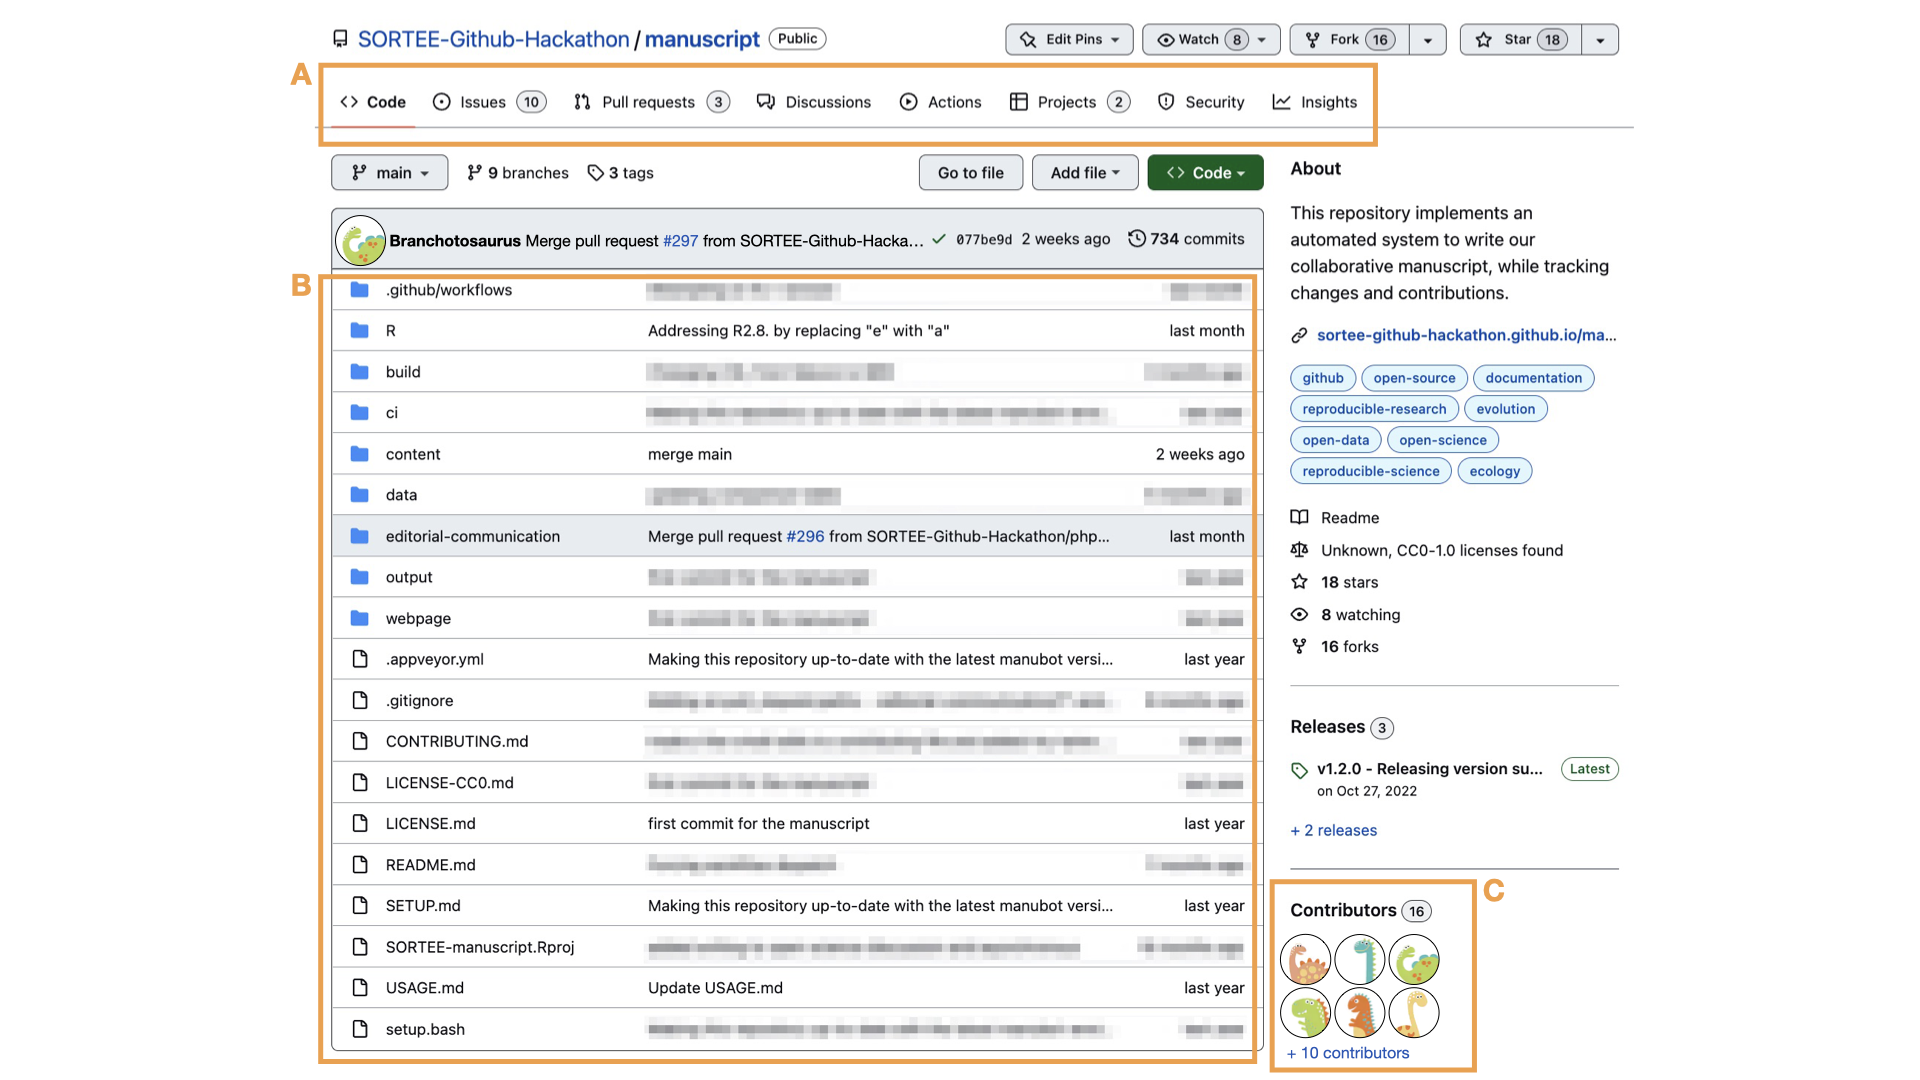
\includegraphics{images/Figure1.png}
\caption{An overview of Git's core features. A) Multi-faceted components allow for code writing, small data storage, manuscript writing, and project management to all be done in one place. \texttt{CONTRIBUTING.md}, \texttt{LICENCE.md}, and \texttt{README.md} files allow new team members, or others wanting to use materials, to understand the project components and learn how they can engage with the project and existing team members. B) Issues, Pull Requests, Discussions, and Projects allow for team members to ask for feedback, suggest fixes, discuss related ideas, and keep track of all the moving parts of a project. C) All collaborators on a project can be a part of a single repository, with varying push privileges and responsibilities.}\label{fig:github-diagram}
}
\end{figure}

\begin{figure}
\hypertarget{fig:scatterblob}{%
\centering
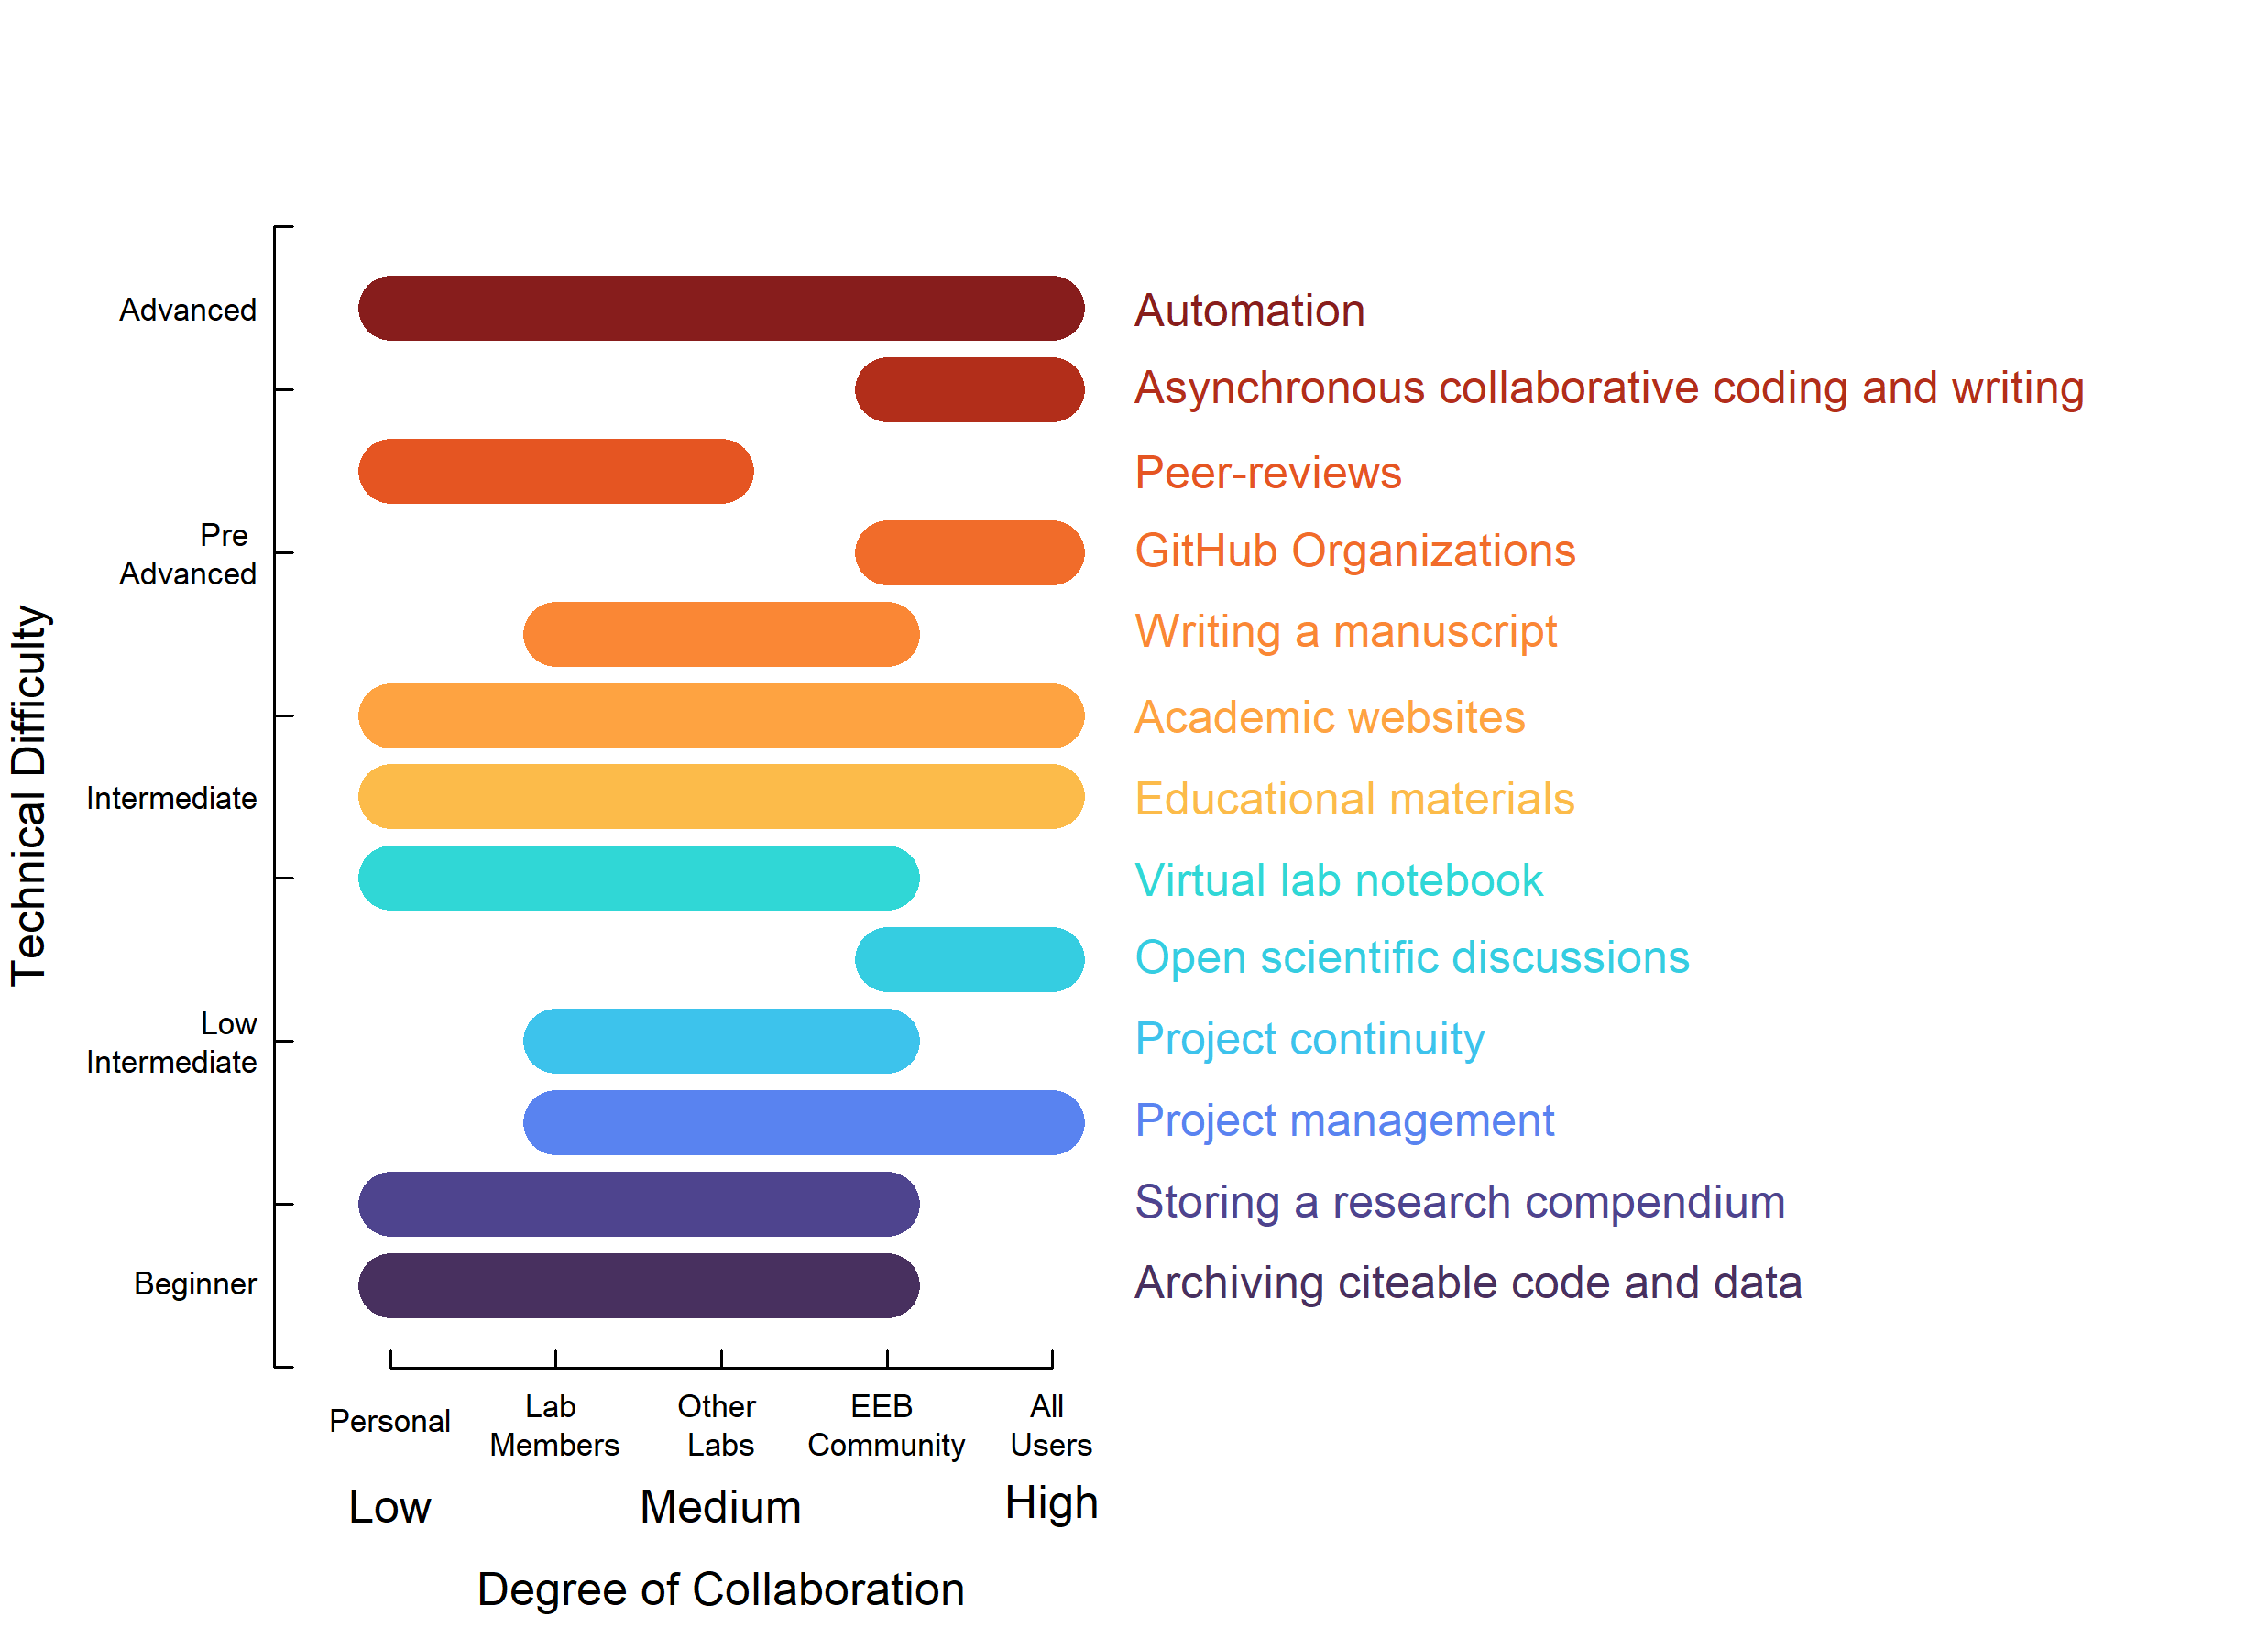
\includegraphics{images/scatterblob_1-viridis-turbo.png}
\caption{A summary of ways GitHub can be used showing technical difficulty and degree of collaboration for each. Activities higher on the vertical axis require usage knowledge of more GitHub features than activities lower on the axis. On the horizontal axis, each activity spans a region representing who is potentially involved with or benefits from each activity. For example, storing data and code mainly benefits individual researchers or members of a lab group while making data and code citable and reproducible benefit other labs and the larger community as well. Independently of a users knowledge level of GitHub features, there are ways to use GitHub that allow tapping unto one of the most salient benefits of the platform: facilitating and enhancing collaboration.}\label{fig:scatterblob}
}
\end{figure}

\hypertarget{tables}{%
\subsection{Tables}\label{tables}}

\begin{longtable}[]{@{}
  >{\raggedright\arraybackslash}p{(\columnwidth - 18\tabcolsep) * \real{0.0627}}
  >{\raggedright\arraybackslash}p{(\columnwidth - 18\tabcolsep) * \real{0.0528}}
  >{\raggedright\arraybackslash}p{(\columnwidth - 18\tabcolsep) * \real{0.0281}}
  >{\raggedright\arraybackslash}p{(\columnwidth - 18\tabcolsep) * \real{0.0281}}
  >{\raggedright\arraybackslash}p{(\columnwidth - 18\tabcolsep) * \real{0.0380}}
  >{\raggedright\arraybackslash}p{(\columnwidth - 18\tabcolsep) * \real{0.0528}}
  >{\raggedright\arraybackslash}p{(\columnwidth - 18\tabcolsep) * \real{0.1799}}
  >{\raggedright\arraybackslash}p{(\columnwidth - 18\tabcolsep) * \real{0.1683}}
  >{\raggedright\arraybackslash}p{(\columnwidth - 18\tabcolsep) * \real{0.2558}}
  >{\raggedright\arraybackslash}p{(\columnwidth - 18\tabcolsep) * \real{0.1337}}@{}}
\caption{A comparison of technologies commonly used for collaborating on research in Ecology and Evolutionary Biology. In the first column, we group platforms for collaboration into broad guilds. The second column lists the platform for collaboration. The remaining columns indicate whether the platform for collaboration includes certain features. \label{tbl:compare}}\tabularnewline
\toprule
\begin{minipage}[b]{\linewidth}\raggedright
Guild
\end{minipage} & \begin{minipage}[b]{\linewidth}\raggedright
Software
\end{minipage} & \begin{minipage}[b]{\linewidth}\raggedright
Version control
\end{minipage} & \begin{minipage}[b]{\linewidth}\raggedright
Backup (cloud)
\end{minipage} & \begin{minipage}[b]{\linewidth}\raggedright
Passive collaboration
\end{minipage} & \begin{minipage}[b]{\linewidth}\raggedright
Active real-time collaboration
\end{minipage} & \begin{minipage}[b]{\linewidth}\raggedright
Free plan available
\end{minipage} & \begin{minipage}[b]{\linewidth}\raggedright
Permanent (DOI)
\end{minipage} & \begin{minipage}[b]{\linewidth}\raggedright
Storage limits
\end{minipage} & \begin{minipage}[b]{\linewidth}\raggedright
GitHub Integration
\end{minipage} \\
\midrule
\endfirsthead
\toprule
\begin{minipage}[b]{\linewidth}\raggedright
Guild
\end{minipage} & \begin{minipage}[b]{\linewidth}\raggedright
Software
\end{minipage} & \begin{minipage}[b]{\linewidth}\raggedright
Version control
\end{minipage} & \begin{minipage}[b]{\linewidth}\raggedright
Backup (cloud)
\end{minipage} & \begin{minipage}[b]{\linewidth}\raggedright
Passive collaboration
\end{minipage} & \begin{minipage}[b]{\linewidth}\raggedright
Active real-time collaboration
\end{minipage} & \begin{minipage}[b]{\linewidth}\raggedright
Free plan available
\end{minipage} & \begin{minipage}[b]{\linewidth}\raggedright
Permanent (DOI)
\end{minipage} & \begin{minipage}[b]{\linewidth}\raggedright
Storage limits
\end{minipage} & \begin{minipage}[b]{\linewidth}\raggedright
GitHub Integration
\end{minipage} \\
\midrule
\endhead
Multi-tool & GitHub & yes & yes & yes & no & Broadly used free version. Advanced features are provided for free to students and education professionals. & A DOI can only be obtained when integrating to other services that can mint DOI (e.g., Zenodo, OSF). & 100MB per file, 500MB per private repository (2GB for paid accounts). 100GB for public repositories. Larger files (up to 2GB) can be attached to releases & N/A \\
Multi-tool & Open Science Framework & yes & yes & yes & yes & yes & yes & 25GB for private projects, up to 5GB per file, plus partner add-ons, 50GB for public projects & yes \\
Long-term (public) data repositories & PANGAEA & yes & yes & yes & no & yes & yes & 10 GB free & no \\
Long-term (public) data repositories & Zenodo & after published & after published & yes & no & yes & yes & 50 GB per dataset & yes \\
Long-term (public) data repositories & Dryad & after published & after published & yes & no & some journals cover cost & yes & 300 GB per publication & Can link to individual files (not entire repository), thus not fully integrated \\
Long-term (public) data repositories & Figshare & yes & yes & yes & no & yes & yes & 20 GB free, up to 5 TB & yes \\
Temporary (personal) drive storage & Google Drive & yes & yes & yes & yes & limited free version \& paid & no & 15GB free, up to 100GB with Google One & yes \\
Temporary (personal) drive storage & Box & limited & yes & yes & yes & no & no & Unlimited total size for subscription & yes \\
Temporary (personal) drive storage & DropBox & limited & yes & yes & yes & limited free version \& paid & no & 2GB free & yes \\
Temporary (personal) drive storage & OneDrive and the Office Suite & yes & yes & yes & yes & limited free version \& paid & no & 5 GB free, up to 1TB paid & yes \\
Collaborative code/text editors & Overleaf (online latex editor) & yes & yes & yes & yes & yes & no & 1MB for individual .tex, 50MB for individual files, unlimited project size & yes \\
Collaborative code/text editors & Jupyter Notebook & yes & ? & yes & with Colab & yes & no & via Binder: no hard limit, but suggests no files \textgreater100MB, can also store on GitHub or Google Colab & yes \\
Collaborative code/text editors & HackMD & yes & yes & yes & yes & limited free version \& paid & no & 3 documents free, private invitee limits & yes \\
\bottomrule
\end{longtable}

\begin{longtable}[]{@{}
  >{\raggedright\arraybackslash}p{(\columnwidth - 14\tabcolsep) * \real{0.0493}}
  >{\raggedright\arraybackslash}p{(\columnwidth - 14\tabcolsep) * \real{0.1425}}
  >{\raggedright\arraybackslash}p{(\columnwidth - 14\tabcolsep) * \real{0.1041}}
  >{\raggedright\arraybackslash}p{(\columnwidth - 14\tabcolsep) * \real{0.1562}}
  >{\raggedright\arraybackslash}p{(\columnwidth - 14\tabcolsep) * \real{0.1096}}
  >{\raggedright\arraybackslash}p{(\columnwidth - 14\tabcolsep) * \real{0.1479}}
  >{\raggedright\arraybackslash}p{(\columnwidth - 14\tabcolsep) * \real{0.1370}}
  >{\raggedright\arraybackslash}p{(\columnwidth - 14\tabcolsep) * \real{0.1534}}@{}}
\caption{A non-exhaustive collection of ideas for how various GitHub
features could be utilized for a research project. Here we have
categorized contributors/collaborators into five roles. A Project
Manager owns the GitHub repository for a project, and leads the academic
project (e.g., lead author of a manuscript). A co-author contributes to
writing and other aspects of research, but may have limited or no
experience with programming, git, and/or GitHub. A code contributor
writes or edits analysis code for the project. A code reviewer could be
a project collaborator or a peer reviewer who reviews project code. They
are familiar with coding, but not necessarily with git or GitHub (but
they are willing to learn). Finally, community members could be other
researchers or non-researchers interested in reproducing results,
re-using code or data, or communicating with researchers involved in the
project. These roles are not mutually exclusive---a co-author could also
be a code contributor and code reviewer, for example. For definitions of
the GitHub features, see Box 1. \label{tbl:roles}}\tabularnewline
\toprule
\begin{minipage}[b]{\linewidth}\raggedright
Role
\end{minipage} & \begin{minipage}[b]{\linewidth}\raggedright
GitHub repository
\end{minipage} & \begin{minipage}[b]{\linewidth}\raggedright
README
\end{minipage} & \begin{minipage}[b]{\linewidth}\raggedright
Issue
\end{minipage} & \begin{minipage}[b]{\linewidth}\raggedright
Discussion
\end{minipage} & \begin{minipage}[b]{\linewidth}\raggedright
Pull Request
\end{minipage} & \begin{minipage}[b]{\linewidth}\raggedright
Fork
\end{minipage} & \begin{minipage}[b]{\linewidth}\raggedright
GitHub Pages
\end{minipage} \\
\midrule
\endfirsthead
\toprule
\begin{minipage}[b]{\linewidth}\raggedright
Role
\end{minipage} & \begin{minipage}[b]{\linewidth}\raggedright
GitHub repository
\end{minipage} & \begin{minipage}[b]{\linewidth}\raggedright
README
\end{minipage} & \begin{minipage}[b]{\linewidth}\raggedright
Issue
\end{minipage} & \begin{minipage}[b]{\linewidth}\raggedright
Discussion
\end{minipage} & \begin{minipage}[b]{\linewidth}\raggedright
Pull Request
\end{minipage} & \begin{minipage}[b]{\linewidth}\raggedright
Fork
\end{minipage} & \begin{minipage}[b]{\linewidth}\raggedright
GitHub Pages
\end{minipage} \\
\midrule
\endhead
Project manager & Set contributor permissions, share code of conduct & Project description, citation, DOIs & Assign tasks to collaborators & Discuss project directions and goals & Approve and incorporate edits to code and/or writing & & Share up-to-date reports, figures, or draft manuscript \\
Co-author & Edit Markdown text or add files & & Propose changes involving code (e.g.~analyses, figures) & Discuss proposed changes to manuscript & & & \\
Code contributor & & & Suggest code changes & & Contribute changes to code, initiate code review & & Contribute to project website \\
Code reviewer & Find all code related to a project & & Highlight specific lines of code and make suggestions & & Review or recommended changes in code & & \\
Community & & & Suggest additional features and report bugs & Ask questions about data and code & & Create a linked, editable copy of the repository & View project website \\
\bottomrule
\end{longtable}

\hypertarget{references}{%
\subsection{References}\label{references}}

\hypertarget{refs}{}
\begin{CSLReferences}{1}{0}
\leavevmode\vadjust pre{\hypertarget{ref-s91uGRZ2}{}}%
\emph{About code owners}. (n.d.). GitHub Docs. Retrieved February 6, 2023, from \url{https://ghdocs-prod.azurewebsites.net/en/repositories/managing-your-repositorys-settings-and-features/customizing-your-repository/about-code-owners}

\leavevmode\vadjust pre{\hypertarget{ref-1Co6ZZjF1}{}}%
\emph{About large files on GitHub}. (n.d.). GitHub Docs. Retrieved February 6, 2023, from \url{https://ghdocs-prod.azurewebsites.net/en/repositories/working-with-files/managing-large-files/about-large-files-on-github}

\leavevmode\vadjust pre{\hypertarget{ref-RhBKe0MG}{}}%
\emph{About Projects}. (n.d.). GitHub Docs. Retrieved February 6, 2023, from \url{https://ghdocs-prod.azurewebsites.net/en/issues/planning-and-tracking-with-projects/learning-about-projects/about-projects}

\leavevmode\vadjust pre{\hypertarget{ref-TOsASkn5}{}}%
\emph{Adding a license to a repository}. (n.d.). GitHub Docs. Retrieved February 6, 2023, from \url{https://ghdocs-prod.azurewebsites.net/en/communities/setting-up-your-project-for-healthy-contributions/adding-a-license-to-a-repository}

\leavevmode\vadjust pre{\hypertarget{ref-13QX8XU3J}{}}%
Alston, J. M., \& Rick, J. A. (2021). A Beginner's Guide to Conducting Reproducible Research. \emph{The Bulletin of the Ecological Society of America}, \emph{102}(2). \url{https://doi.org/10.1002/bes2.1801}

\leavevmode\vadjust pre{\hypertarget{ref-UsTxAq4f}{}}%
Anbaroğlu, B. (2021). A collaborative GIS programming course using GitHub Classroom. \emph{Transactions in GIS}, \emph{25}(6), 3132--3158. \url{https://doi.org/10.1111/tgis.12810}

\leavevmode\vadjust pre{\hypertarget{ref-1HZdsK5Kn}{}}%
Baker, M. (2016). 1,500 scientists lift the lid on reproducibility. \emph{Nature}, \emph{533}(7604), 452--454. \url{https://doi.org/10.1038/533452a}

\leavevmode\vadjust pre{\hypertarget{ref-Qh7xTLwz}{}}%
Beaulieu-Jones, B. K., \& Greene, C. S. (2017). Reproducibility of computational workflows is automated using continuous analysis. \emph{Nature Biotechnology}, \emph{35}(4), 342--346. \url{https://doi.org/10.1038/nbt.3780}

\leavevmode\vadjust pre{\hypertarget{ref-PlcxShQU}{}}%
Blischak, J. D., Davenport, E. R., \& Wilson, G. (2016). A Quick Introduction to Version Control with Git and GitHub. \emph{PLOS Computational Biology}, \emph{12}(1), e1004668. \url{https://doi.org/10.1371/journal.pcbi.1004668}

\leavevmode\vadjust pre{\hypertarget{ref-Xsdcv6q}{}}%
Boettiger, C., Lang, D. T., \& Wainwright, P. C. (2012). rfishbase: exploring, manipulating and visualizing FishBase data from R. \emph{Journal of Fish Biology}, \emph{81}(6), 2030--2039. \url{https://doi.org/10.1111/j.1095-8649.2012.03464.x}

\leavevmode\vadjust pre{\hypertarget{ref-gLby7jt1}{}}%
Borghi, J., \& Van Gulick, A. (2022). Promoting Open Science Through Research Data Management. \emph{Harvard Data Science Review}. \url{https://doi.org/10.1162/99608f92.9497f68e}

\leavevmode\vadjust pre{\hypertarget{ref-ydrk01SR}{}}%
Briney, K., Coates, H., \& Goben, A. (2020). Foundational Practices of Research Data Management. \emph{Research Ideas and Outcomes}, \emph{6}. \url{https://doi.org/10.3897/rio.6.e56508}

\leavevmode\vadjust pre{\hypertarget{ref-RVetqmsg}{}}%
Bryan, J. (2018). Excuse Me, Do You Have a Moment to Talk About Version Control? \emph{The American Statistician}, \emph{72}(1), 20--27. \url{https://doi.org/10.1080/00031305.2017.1399928}

\leavevmode\vadjust pre{\hypertarget{ref-6CMMeSeD}{}}%
Bryan, J., \& TAs, T. S. 545. (n.d.). \emph{STAT 545}. Retrieved February 6, 2023, from \url{https://stat545.com/}

\leavevmode\vadjust pre{\hypertarget{ref-FVBWKkZu}{}}%
Chamberlain, S. A., \& Szöcs, E. (2013). taxize: taxonomic search and retrieval in R. \emph{F1000Research}, \emph{2}, 191. \url{https://doi.org/10.12688/f1000research.2-191.v2}

\leavevmode\vadjust pre{\hypertarget{ref-lx49NGto}{}}%
\emph{Connect GitHub to a Project - OSF Support}. (n.d.). Retrieved February 6, 2023, from \url{https://help.osf.io/article/211-connect-github-to-a-project}

\leavevmode\vadjust pre{\hypertarget{ref-T03Api6e}{}}%
\emph{Continuous Integration and Delivery}. (n.d.). CircleCI. Retrieved February 6, 2023, from \url{https://circleci.com/}

\leavevmode\vadjust pre{\hypertarget{ref-K7nbP1Ty}{}}%
Crystal-Ornelas, R., Edwards, B. P. M., Hébert, K., Hudgins, E. J., Reyes, L. L. S., Scott, E. R., Grainger, M. J., Foroughirad, V., Binley, A. D., Brookson, C. B., Gaynor, K. M., Sabet, S. S., Güncan, A., Hillemann, F., Weierbach, H., Gomes, D. G. E., \& Braga, P. H. P. (2023). \emph{Not just for programmers: How GitHub can accelerate collaborative and reproducible research in ecology and evolution}. Manubot. \url{https://SORTEE-Github-Hackathon.github.io/manuscript/}

\leavevmode\vadjust pre{\hypertarget{ref-1Du6fzB8g}{}}%
Crystal‐Ornelas, R., Varadharajan, C., Bond‐Lamberty, B., Boye, K., Burrus, M., Cholia, S., Crow, M., Damerow, J., Devarakonda, R., Ely, K. S., Goldman, A., Heinz, S., Hendrix, V., Kakalia, Z., Pennington, S. C., Robles, E., Rogers, A., Simmonds, M., Velliquette, T., \ldots{} Agarwal, D. A. (2021). A Guide to Using GitHub for Developing and Versioning Data Standards and Reporting Formats. \emph{Earth and Space Science}, \emph{8}(8). \url{https://doi.org/10.1029/2021ea001797}

\leavevmode\vadjust pre{\hypertarget{ref-NOgBWVAr}{}}%
Culina, A., van den Berg, I., Evans, S., \& Sánchez-Tójar, A. (2020). Low availability of code in ecology: A~call for urgent action. \emph{PLOS Biology}, \emph{18}(7), e3000763. \url{https://doi.org/10.1371/journal.pbio.3000763}

\leavevmode\vadjust pre{\hypertarget{ref-rTbinQMj}{}}%
Dietze, M. C., Fox, A., Beck-Johnson, L. M., Betancourt, J. L., Hooten, M. B., Jarnevich, C. S., Keitt, T. H., Kenney, M. A., Laney, C. M., Larsen, L. G., Loescher, H. W., Lunch, C. K., Pijanowski, B. C., Randerson, J. T., Read, E. K., Tredennick, A. T., Vargas, R., Weathers, K. C., \& White, E. P. (2018). Iterative near-term ecological forecasting: Needs, opportunities, and challenges. \emph{Proceedings of the National Academy of Sciences}, \emph{115}(7), 1424--1432. \url{https://doi.org/10.1073/pnas.1710231115}

\leavevmode\vadjust pre{\hypertarget{ref-bZNn2hbh}{}}%
EllenJCoombs. (2020). \emph{EllenJCoombs/Asymmetry-evolution-cetaceans-for-publication-v.1.0.0} (Version v.1.0.0) {[}Computer software{]}. Zenodo. \url{https://doi.org/10.5281/zenodo.3893943}

\leavevmode\vadjust pre{\hypertarget{ref-RxK4CmfR}{}}%
Ernest, S. K. M., Yenni, G. M., Allington, G., Bledsoe, E. K., Christensen, E. M., Diaz, R. M., Geluso, K., Goheen, J. R., Guo, Q., Heske, E., Kelt, D., Meiners, J. M., Munger, J., Restrepo, C., Samson, D. A., Schutzenhofer, M. R., Skupski, M., Supp, S. R., Thibault, K., \ldots{} Valone, T. J. (2018). \emph{The Portal Project: a long-term study of a Chihuahuan desert ecosystem}. Cold Spring Harbor Laboratory. \url{https://doi.org/10.1101/332783}

\leavevmode\vadjust pre{\hypertarget{ref-NUXbp429}{}}%
\emph{Features • GitHub Actions}. (n.d.). GitHub. Retrieved February 6, 2023, from \url{https://github.com/features/actions}

\leavevmode\vadjust pre{\hypertarget{ref-D4C4k4ak}{}}%
Fehr, J., Himpe, C., Rave, S., \& Saak, J. (2021). Sustainable Research Software Hand-Over. \emph{Journal of Open Research Software}, \emph{9}(1), 5. \url{https://doi.org/10.5334/jors.307}

\leavevmode\vadjust pre{\hypertarget{ref-SLq38RVv}{}}%
Figueiredo, A. S. (2017). Data Sharing: Convert Challenges into Opportunities. \emph{Frontiers in Public Health}, \emph{5}. \url{https://doi.org/10.3389/fpubh.2017.00327}

\leavevmode\vadjust pre{\hypertarget{ref-1CM2EcdVk}{}}%
\emph{Git - A Short History of Git}. (n.d.). Retrieved February 6, 2023, from \url{https://git-scm.com/book/en/v2/Getting-Started-A-Short-History-of-Git}

\leavevmode\vadjust pre{\hypertarget{ref-VDJput1V}{}}%
Gomes, D. G. E., Pottier, P., Crystal-Ornelas, R., Hudgins, E. J., Foroughirad, V., Sánchez-Reyes, L. L., Turba, R., Martinez, P. A., Moreau, D., Bertram, M. G., Smout, C. A., \& Gaynor, K. M. (2022a). Why don't we share data and code? Perceived barriers and benefits to public archiving practices. \emph{Proceedings of the Royal Society B: Biological Sciences}, \emph{289}(1987). \url{https://doi.org/10.1098/rspb.2022.1113}

\leavevmode\vadjust pre{\hypertarget{ref-pq2Tv1BC}{}}%
Gomes, D. G. E., Pottier, P., Crystal-Ornelas, R., Hudgins, E. J., Foroughirad, V., Sánchez-Reyes, L. L., Turba, R., Martinez, P. A., Moreau, D., Bertram, M., Smout, C., \& Gaynor, K. (2022b). \emph{Why don't we share data and code? Perceived barriers and benefits to public archiving practices}. Center for Open Science. \url{https://doi.org/10.31222/osf.io/gaj43}

\leavevmode\vadjust pre{\hypertarget{ref-1HhzKAC1K}{}}%
Goring, S. J., Weathers, K. C., Dodds, W. K., Soranno, P. A., Sweet, L. C., Cheruvelil, K. S., Kominoski, J. S., Rüegg, J., Thorn, A. M., \& Utz, R. M. (2014). Improving the culture of interdisciplinary collaboration in ecology by expanding measures of success. \emph{Frontiers in Ecology and the Environment}, \emph{12}(1), 39--47. \url{https://doi.org/10.1890/120370}

\leavevmode\vadjust pre{\hypertarget{ref-iIEKCTLU}{}}%
Hampton, S. E., Anderson, S. S., Bagby, S. C., Gries, C., Han, X., Hart, E. M., Jones, M. B., Lenhardt, W. C., MacDonald, A., Michener, W. K., Mudge, J., Pourmokhtarian, A., Schildhauer, M. P., Woo, K. H., \& Zimmerman, N. (2015). The Tao of open science for ecology. \emph{Ecosphere}, \emph{6}(7), art120. \url{https://doi.org/10.1890/es14-00402.1}

\leavevmode\vadjust pre{\hypertarget{ref-fJWFe93e}{}}%
Hannay, J. E., MacLeod, C., Singer, J., Langtangen, H. P., Pfahl, D., \& Wilson, G. (2009, May). How do scientists develop and use scientific software? \emph{2009 ICSE Workshop on Software Engineering for Computational Science and Engineering}. 2009 ICSE Workshop on Software Engineering for Computational Science and Engineering (SECSE). \url{https://doi.org/10.1109/secse.2009.5069155}

\leavevmode\vadjust pre{\hypertarget{ref-ZvrOcg9w}{}}%
Hester, J. B., the STAT 545 TAs, Jim. (n.d.). \emph{Let's Git started \textbar{} Happy Git and GitHub for the useR}. Retrieved February 6, 2023, from \url{https://happygitwithr.com/}

\leavevmode\vadjust pre{\hypertarget{ref-YuJbg3zO}{}}%
Himmelstein, D. S., Rubinetti, V., Slochower, D. R., Hu, D., Malladi, V. S., Greene, C. S., \& Gitter, A. (2019). Open collaborative writing with Manubot. \emph{PLOS Computational Biology}, \emph{15}(6), e1007128. \url{https://doi.org/10.1371/journal.pcbi.1007128}

\leavevmode\vadjust pre{\hypertarget{ref-YeFSbfFV}{}}%
\emph{Home -- Travis-CI}. (2022, October 6). \url{https://www.travis-ci.com/}

\leavevmode\vadjust pre{\hypertarget{ref-GQj3c17f}{}}%
Hudgins, E. (2022). \emph{emmajhudgins/UStreedamage: publication release} (accepted) {[}Computer software{]}. Zenodo. \url{https://doi.org/10.5281/zenodo.6097109}

\leavevmode\vadjust pre{\hypertarget{ref-3UAritXO}{}}%
\emph{Issues · fmsabatini/sPlotOpen\_Manuscript}. (n.d.). GitHub. Retrieved February 6, 2023, from \url{https://github.com/fmsabatini/sPlotOpen_Manuscript}

\leavevmode\vadjust pre{\hypertarget{ref-ndfO9H}{}}%
Kalliamvakou, E., Damian, D., Blincoe, K., Singer, L., \& German, D. M. (2015, May). Open Source-Style Collaborative Development Practices in Commercial Projects Using GitHub. \emph{2015 IEEE/ACM 37th IEEE International Conference on Software Engineering}. 2015 IEEE/ACM 37th IEEE International Conference on Software Engineering (ICSE). \url{https://doi.org/10.1109/icse.2015.74}

\leavevmode\vadjust pre{\hypertarget{ref-cfgXxgt1}{}}%
Keitt, T. H., \& Abelson, E. S. (2021). Ecology in the age of automation. \emph{Science}, \emph{373}(6557), 858--859. \url{https://doi.org/10.1126/science.abi4692}

\leavevmode\vadjust pre{\hypertarget{ref-cW7vGddM}{}}%
Khelifa, R., Amano, T., \& Nuñez, M. A. (2022). A solution for breaking the language barrier. \emph{Trends in Ecology \&Amp; Evolution}, \emph{37}(2), 109--112. \url{https://doi.org/10.1016/j.tree.2021.11.003}

\leavevmode\vadjust pre{\hypertarget{ref-lJAgyhYq}{}}%
Kim, A. Y., Herrmann, V., Barreto, R., Calkins, B., Gonzalez‐Akre, E., Johnson, D. J., Jordan, J. A., Magee, L., McGregor, I. R., Montero, N., Novak, K., Rogers, T., Shue, J., \& Anderson‐Teixeira, K. J. (2022). Implementing GitHub Actions continuous integration to reduce error rates in ecological data collection. \emph{Methods in Ecology and Evolution}, \emph{13}(11), 2572--2585. \url{https://doi.org/10.1111/2041-210x.13982}

\leavevmode\vadjust pre{\hypertarget{ref-139b0pSGc}{}}%
Leibzon, W. (2016, August). Social network of software development at GitHub. \emph{2016 IEEE/ACM International Conference on Advances in Social Networks Analysis and Mining (ASONAM)}. 2016 IEEE/ACM International Conference on Advances in Social Networks Analysis and Mining (ASONAM). \url{https://doi.org/10.1109/asonam.2016.7752419}

\leavevmode\vadjust pre{\hypertarget{ref-3DKwn1sY}{}}%
Lowndes, J. S. S., Best, B. D., Scarborough, C., Afflerbach, J. C., Frazier, M. R., O'Hara, C. C., Jiang, N., \& Halpern, B. S. (2017). Our path to better science in less time using open data science tools. \emph{Nature Ecology \&Amp; Evolution}, \emph{1}(6). \url{https://doi.org/10.1038/s41559-017-0160}

\leavevmode\vadjust pre{\hypertarget{ref-ZI1OqZNr}{}}%
Lrharper1. (2018). \emph{Hulluni-Bioinformatics/Harper\_Et\_Al\_2018: Github Repository Deposited With Harper Et Al. (2018) In Ecology And Evolution.} Zenodo. \url{https://doi.org/10.5281/zenodo.1188710}

\leavevmode\vadjust pre{\hypertarget{ref-pjy75gHr}{}}%
Madicken Munk, Koziar, K., Leinweber, K., Raniere Silva, Michonneau, F., McCue, R., Hejazi, N., Waldman, S., Emonet, R., Harris, R. M., Olex, A. L., Becker, E. A., Lever, J., Burle, M.-H., Moore, B., Umihiko Hoshijima, Maji, A., Topçuoğlu, B. D., Junghans, C., \ldots{} Wolmar Nyberg Åkerström. (2019). \emph{swcarpentry/git-novice: Software Carpentry: Version Control with Git, June 2019} (Version v2019.06.1). Zenodo. \url{https://doi.org/10.5281/zenodo.3264950}

\leavevmode\vadjust pre{\hypertarget{ref-Re6Eg2va}{}}%
\emph{Manubot - Manuscripts, open and automated}. (n.d.). Retrieved February 6, 2023, from \url{https://manubot.org}

\leavevmode\vadjust pre{\hypertarget{ref-MwwMapRG}{}}%
Marwick, B., Boettiger, C., \& Mullen, L. (2018). Packaging Data Analytical Work Reproducibly Using R (and Friends). \emph{The American Statistician}, \emph{72}(1), 80--88. \url{https://doi.org/10.1080/00031305.2017.1375986}

\leavevmode\vadjust pre{\hypertarget{ref-mmCOSRfr}{}}%
McIntire, E. J. B., Chubaty, A. M., Cumming, S. G., Andison, D., Barros, C., Boisvenue, C., Haché, S., Luo, Y., Micheletti, T., \& Stewart, F. E. C. (2022). PERFICT: A Re‐imagined foundation for predictive ecology. \emph{Ecology Letters}, \emph{25}(6), 1345--1351. \url{https://doi.org/10.1111/ele.13994}

\leavevmode\vadjust pre{\hypertarget{ref-1Ep9EJL6y}{}}%
Meyer, M. (2014). Continuous Integration and Its Tools. \emph{IEEE Software}, \emph{31}(3), 14--16. \url{https://doi.org/10.1109/ms.2014.58}

\leavevmode\vadjust pre{\hypertarget{ref-bhDgD6lF}{}}%
Micheletti, T., Stewart, F. E. C., Cumming, S. G., Haché, S., Stralberg, D., Tremblay, J. A., Barros, C., Eddy, I. M. S., Chubaty, A. M., Leblond, M., Pankratz, R. F., Mahon, C. L., Van Wilgenburg, S. L., Bayne, E. M., Schmiegelow, F., \& McIntire, E. J. B. (2021). Assessing Pathways of Climate Change Effects in SpaDES: An Application to Boreal Landbirds of Northwest Territories Canada. \emph{Frontiers in Ecology and Evolution}, \emph{9}. \url{https://doi.org/10.3389/fevo.2021.679673}

\leavevmode\vadjust pre{\hypertarget{ref-uBJwnPbq}{}}%
Mislan, K. A. S., Heer, J. M., \& White, E. P. (2016). Elevating The Status of Code in Ecology. \emph{Trends in Ecology \&Amp; Evolution}, \emph{31}(1), 4--7. \url{https://doi.org/10.1016/j.tree.2015.11.006}

\leavevmode\vadjust pre{\hypertarget{ref-kZzfmBNu}{}}%
Naujokaitis-Lewis, I., Endicott, S., \& Guezen, J. M. (2022). CAN-SAR: A database of Canadian species at risk information. \emph{Scientific Data}, \emph{9}(1). \url{https://doi.org/10.1038/s41597-022-01381-8}

\leavevmode\vadjust pre{\hypertarget{ref-1Hcf13Q0k}{}}%
Nugroho, R. P., Zuiderwijk, A., Janssen, M., \& de Jong, M. (2015). A comparison of national open data policies: lessons learned. \emph{Transforming Government: People, Process and Policy}, \emph{9}(3), 286--308. \url{https://doi.org/10.1108/tg-03-2014-0008}

\leavevmode\vadjust pre{\hypertarget{ref-4LaijDIZ}{}}%
On data availability, reproducibility and reuse. (2017). \emph{Nature Cell Biology}, \emph{19}(4), 259--259. \url{https://doi.org/10.1038/ncb3506}

\leavevmode\vadjust pre{\hypertarget{ref-kEX5dgzK}{}}%
Perez-Riverol, Y., Gatto, L., Wang, R., Sachsenberg, T., Uszkoreit, J., Leprevost, F. da V., Fufezan, C., Ternent, T., Eglen, S. J., Katz, D. S., Pollard, T. J., Konovalov, A., Flight, R. M., Blin, K., \& Vizcaíno, J. A. (2016). Ten Simple Rules for Taking Advantage of Git and GitHub. \emph{PLOS Computational Biology}, \emph{12}(7), e1004947. \url{https://doi.org/10.1371/journal.pcbi.1004947}

\leavevmode\vadjust pre{\hypertarget{ref-10ghgV3S8}{}}%
Perkel, J. (2016). Democratic databases: science on GitHub. \emph{Nature}, \emph{538}(7623), 127--128. \url{https://doi.org/10.1038/538127a}

\leavevmode\vadjust pre{\hypertarget{ref-1Kqna6l2}{}}%
Perkel, J. M. (2020). Challenge to scientists: does your ten-year-old code still run? \emph{Nature}, \emph{584}(7822), 656--658. \url{https://doi.org/10.1038/d41586-020-02462-7}

\leavevmode\vadjust pre{\hypertarget{ref-1CcAUn3Lu}{}}%
Piwowar, H. A., Day, R. S., \& Fridsma, D. B. (2007). Sharing Detailed Research Data Is Associated with Increased Citation Rate. \emph{PLoS ONE}, \emph{2}(3), e308. \url{https://doi.org/10.1371/journal.pone.0000308}

\leavevmode\vadjust pre{\hypertarget{ref-666HppfO}{}}%
Pronk, T. E., Wiersma, P. H., van Weerden, A., \& Schieving, F. (2015). A game theoretic analysis of research data sharing. \emph{PeerJ}, \emph{3}, e1242. \url{https://doi.org/10.7717/peerj.1242}

\leavevmode\vadjust pre{\hypertarget{ref-4ny1onB0}{}}%
Ram, K. (2013). Git can facilitate greater reproducibility and increased transparency in science. \emph{Source Code for Biology and Medicine}, \emph{8}(1). \url{https://doi.org/10.1186/1751-0473-8-7}

\leavevmode\vadjust pre{\hypertarget{ref-12103x16N}{}}%
Scheller, R. M., Sturtevant, B. R., Gustafson, E. J., Ward, B. C., \& Mladenoff, D. J. (2010). Increasing the reliability of ecological models using modern software engineering techniques. \emph{Frontiers in Ecology and the Environment}, \emph{8}(5), 253--260. \url{https://doi.org/10.1890/080141}

\leavevmode\vadjust pre{\hypertarget{ref-HiIPSSHV}{}}%
Smaglik, P. (2007). Creating better lab websites gives potential collaborators and recruiters a clearer window into your world. \emph{Nature}, \emph{447}(7142), 347--347. \url{https://doi.org/10.1038/nj7142-347a}

\leavevmode\vadjust pre{\hypertarget{ref-ufw0ZdnI}{}}%
Soergel, D. A. W. (2015). Rampant software errors may undermine scientific results. \emph{F1000Research}, \emph{3}, 303. \url{https://doi.org/10.12688/f1000research.5930.2}

\leavevmode\vadjust pre{\hypertarget{ref-hm9PaCLD}{}}%
Song, X., Goldstein, S. C., \& Sakr, M. (2020, June 15). Using Peer Code Review as an Educational Tool. \emph{Proceedings of the 2020 ACM Conference on Innovation and Technology in Computer Science Education}. ITiCSE '20: Innovation and Technology in Computer Science Education. \url{https://doi.org/10.1145/3341525.3387370}

\leavevmode\vadjust pre{\hypertarget{ref-7q3wZN6d}{}}%
Spinellis, D. (2012). Git. \emph{IEEE Software}, \emph{29}(3), 100--101. \url{https://doi.org/10.1109/ms.2012.61}

\leavevmode\vadjust pre{\hypertarget{ref-1CzUZwyU2}{}}%
Tenopir, C., Dalton, E. D., Allard, S., Frame, M., Pjesivac, I., Birch, B., Pollock, D., \& Dorsett, K. (2015). Changes in Data Sharing and Data Reuse Practices and Perceptions among Scientists Worldwide. \emph{PLOS ONE}, \emph{10}(8), e0134826. \url{https://doi.org/10.1371/journal.pone.0134826}

\leavevmode\vadjust pre{\hypertarget{ref-PLmDFZrm}{}}%
Tenopir, C., Rice, N. M., Allard, S., Baird, L., Borycz, J., Christian, L., Grant, B., Olendorf, R., \& Sandusky, R. J. (2020). Data sharing, management, use, and reuse: Practices and perceptions of scientists worldwide. \emph{PLOS ONE}, \emph{15}(3), e0229003. \url{https://doi.org/10.1371/journal.pone.0229003}

\leavevmode\vadjust pre{\hypertarget{ref-dqrFjoSb}{}}%
Trujillo, G., \& Tanner, K. D. (2014). Considering the Role of Affect in Learning: Monitoring Students' Self-Efficacy, Sense of Belonging, and Science Identity. \emph{CBE---Life Sciences Education}, \emph{13}(1), 6--15. \url{https://doi.org/10.1187/cbe.13-12-0241}

\leavevmode\vadjust pre{\hypertarget{ref-oGbKxHzj}{}}%
\emph{Using Git and GitHub}. (n.d.). Retrieved February 6, 2023, from \url{https://www.overleaf.com/learn/how-to/Using_Git_and_GitHub}

\leavevmode\vadjust pre{\hypertarget{ref-1BJcvyTmV}{}}%
Vale, G., Schmid, A., Santos, A. R., de Almeida, E. S., \& Apel, S. (2019). On the relation between Github communication activity and merge conflicts. \emph{Empirical Software Engineering}, \emph{25}(1), 402--433. \url{https://doi.org/10.1007/s10664-019-09774-x}

\leavevmode\vadjust pre{\hypertarget{ref-19kmNxiHc}{}}%
Vines, Timothy~H., Albert, Arianne~Y. K., Andrew, Rose~L., Débarre, F., Bock, Dan~G., Franklin, Michelle~T., Gilbert, Kimberly~J., Moore, J.-S., Renaut, S., \& Rennison, Diana~J. (2014). The Availability of Research Data Declines Rapidly with Article Age. \emph{Current Biology}, \emph{24}(1), 94--97. \url{https://doi.org/10.1016/j.cub.2013.11.014}

\leavevmode\vadjust pre{\hypertarget{ref-SirQKFIz}{}}%
White, E. P., Yenni, G. M., Taylor, S. D., Christensen, E. M., Bledsoe, E. K., Simonis, J. L., \& Ernest, S. K. M. (2018). Developing an automated iterative near‐term forecasting system for an ecological study. \emph{Methods in Ecology and Evolution}, \emph{10}(3), 332--344. \url{https://doi.org/10.1111/2041-210x.13104}

\leavevmode\vadjust pre{\hypertarget{ref-1Ch6LSHef}{}}%
Wicherts, J. M., Bakker, M., \& Molenaar, D. (2011). Willingness to Share Research Data Is Related to the Strength of the Evidence and the Quality of Reporting of Statistical Results. \emph{PLoS ONE}, \emph{6}(11), e26828. \url{https://doi.org/10.1371/journal.pone.0026828}

\leavevmode\vadjust pre{\hypertarget{ref-1CJo8lo2v}{}}%
Yenni, G. M., Christensen, E. M., Bledsoe, E. K., Supp, S. R., Diaz, R. M., White, E. P., \& Ernest, S. K. M. (2019). Developing a modern data workflow for regularly updated data. \emph{PLOS Biology}, \emph{17}(1), e3000125. \url{https://doi.org/10.1371/journal.pbio.3000125}

\leavevmode\vadjust pre{\hypertarget{ref-lXvpQxeN}{}}%
Yenni, G. M., Christensen, E. M., Bledsoe, E. K., Supp, S. R., Diaz, R. M., White, E. P., \& Ernest, S. K. M. (2018). \emph{Developing a modern data workflow for evolving data}. Cold Spring Harbor Laboratory. \url{https://doi.org/10.1101/344804}

\end{CSLReferences}
